\documentclass[12pt]{report}
\usepackage{listings}
\usepackage{xcolor}

\definecolor{codegreen}{rgb}{0,0.6,0}
\definecolor{codegray}{rgb}{0.5,0.5,0.5}
\definecolor{codepurple}{rgb}{0.58,0,0.82}
\definecolor{backcolour}{rgb}{0.95,0.95,0.92}

\definecolor{codebackground}{rgb}{1,1,1} % Color blanco para el fondo

\lstset{
	language=Python,
	basicstyle=\ttfamily\normalsize,
	keywordstyle=\color{blue},
	commentstyle=\color{gray},
	backgroundcolor=\color{codebackground},
	frame=single, % Sin marco
	breaklines=true,
	showstringspaces=false,
	 numbers=left, % Los números de línea aparecerán a la izquierda
	numberstyle=\tiny\color{gray}, % Estilo de los números de línea
	stepnumber=1, % Los números se incrementarán de uno en uno
	numbersep=5pt, % Separación entre el código y los números de línea
}


% Paquetes necesarios
\usepackage[utf8]{inputenc} % Codificación UTF-8
\usepackage[spanish]{babel} % Idioma español
\usepackage{graphicx}       % Para incluir imágenes
\usepackage{hyperref}
\usepackage{array} % Para ajustar espacios en tablas

%\usepackage[all]{hypcap} % Hipervínculos
\usepackage{geometry}       % Configurar márgenes
\usepackage{titlesec}       % Modificar títulos
\usepackage{fancyhdr}       % Encabezados y pies de página
\usepackage{gensymb}
\usepackage{textcomp}
\usepackage{upquote}
\usepackage{svg}
%\setlength{\parindent}{1.5em}
% Configuración de márgenes
\setlength{\tabcolsep}{3pt} % Reduce el espacio horizontal entre texto y barras
\geometry{a4paper, margin=1in}
\graphicspath{{img/}}
\addto\captionsspanish{\renewcommand{\tablename}{Tabla}}
\addto\captionsspanish{\renewcommand{\listtablename}{Índice de Tablas}}

% Configuración de hipervínculos

\hypersetup{
    colorlinks=true,
    linkcolor=blue,
    urlcolor=blue,
    citecolor=blue,
    pdftitle={Título de la Tesis},
    pdfauthor={Tu Nombre}
}

% Configuración del encabezado y pie de página
%\pagestyle{fancy}
%\fancyhf{}
%\fancyhead[L]{Título de la Tesis}
%\fancyhead[R]{\thepage}
%\fancyfoot[C]{Nombre del Autor}

% Configuración de los títulos
\titleformat{\chapter}[hang]{\bfseries\Large}{\thechapter.}{1em}{}

% Inicio del documento

% Inicio del documento
\begin{document}

% Portada
\begin{titlepage}
    \centering
    {\Huge {Universidad de la Habana}}\\[1cm]
    {\Huge {Facultad de Matemática y Computación }}\\[0.5cm]
 
    \begin{figure}[h]
    	\centering
    	
\includegraphics[width=0.3\textwidth]{logoUH.png}
    	
    	
    \end{figure}
    {\noindent\hrulefill}\\[0.2cm]
    
    {\Large\textbf{{\textit{Test} para detectar patrones DIAG y LINE  en las contraseñas gráficas de PassPoint, basado en el promedio de los ángulos máximos de los triángulos de Delaunay, condicionado al número de triángulos }}}\\[0.1cm]
    {\noindent\hrulefill}\\[1.0cm]
    \begin{minipage}{0.8\textwidth}
    \begin{center}
    	{\Large Trabajo de Diploma presentado en opción al título de Licenciado en Ciencias de la Computación}
    	
    \end{center}
    \end{minipage}\\[1cm]
    
    
 
    
    {\Large {Autor: Ovidio Navarro Pazos}}\\[2cm]
   	{\Large {Tutores: M.Sc. Lisset Suárez Plasencia}}\\
   	\hspace{7.5em}{\Large{Dr.C. Carlos Miguel Legón Pérez}}\\
   	\hspace{7.5em}{\Large{M.Sc. Joaquín A. Herrera Macías}}\\
   	[2.0cm]
   	
   	{\large{La Habana, Cuba}}\\
    {\large  \today}
\end{titlepage}




\chapter*{Resumen}
\hypertarget{Resumen}{}

	Un método de autenticación que difiere de las contraseñas alfanuméricas tradicionales es la autenticación gráfica. Una de las técnicas más valiosas dentro de este campo es PassPoint, conocida por su equilibrio entre seguridad y usabilidad. Sin embargo, esta técnica puede ser vulnerada si el usuario sigue patrones predefinidos al seleccionar los cinco puntos en la imagen, como los patrones DIAG y LINE. Investigaciones previas han destacado la utilidad de las características de las triangulaciones de Delaunay para extraer información de estos puntos que constituyen la contraseña, siendo el AMADT (promedio de los ángulos máximos de los triángulos de Delaunay) una de estas características relevantes.
	
	En este estudio, se comparan contraseñas gráficas generadas por la elección aleatoria de cinco puntos en una imagen con contraseñas que siguen patrones específicos del tipo DIAG y LINE. La comparativa se basa en segmentar las contraseñas que siguen estos patrones, considerando el número de triángulos en sus triangulaciones de Delaunay (3, 4 o 5). Experimentalmente se demuestra que, para cada número de triángulos, las contraseñas con patrones DIAG y LINE tienen un AMADT más alto que aquellas generadas con puntos aleatorios. Estudios previos respaldan este resultado y sugieren la viabilidad de un \textit{test} de aleatoriedad espacial para identificar contraseñas gráficas débiles que sigan los patrones DIAG y LINE, utilizando el AMADT como estadígrafo. Se estiman las distribuciones más adecuadas para cada número de triángulos, se implementa un \textit{test} de hipótesis y se valida mediante la estimación de los errores de tipo I y II. La relevancia de este \textit{test} radica en la similitud de los resultados con pruebas previas. Sería crucial determinar si estos hallazgos son redundantes o complementarios para mejorar la seguridad del sistema de autenticación gráfica PassPoint.


\chapter*{Abstract}
\hypertarget{Abstract}{}
	
	One authentication method that differs from traditional alphanumeric passwords is graphical authentication. One of the most valuable techniques within this field is PassPoint, known for its balance between security and usability. However, this technique can be breached if the user follows predefined patterns when selecting the five dots in the image, such as the DIAG and LINE patterns. Previous research has highlighted the usefulness of Delaunay triangulation features to extract information from these points that constitute the password, with AMADT (average of the maximum angles of the Delaunay triangles) being one of these relevant features.
	
	In this study, graphical passwords generated by randomly choosing five points in an image are compared with passwords that follow specific patterns of the DIAG and LINE type. The comparison is based on segmenting the passwords that follow these patterns, considering the number of triangles in their Delaunay triangulations (3, 4 or 5). Experimentally it is shown that, for each number of triangles, passwords with DIAG and LINE patterns have a higher AMADT than those generated with random dots. Previous studies support this result and suggest the feasibility of a spatial randomization test to identify weak graphical passwords following DIAG and LINE patterns, using the AMADT as a statistician. The best-fitting distributions for each number of triangles are estimated, a hypothesis test is implemented and validated by estimating type I and II errors. The relevance of this test lies in the similarity of the results with previous tests. It would be crucial to determine whether these findings are redundant or complementary to improve the security of the PassPoint graphical authentication system.


% Índice
\tableofcontents
\newpage
\listoffigures
\newpage
\listoftables


% Capítulos
\chapter*{\LARGE{Introducción}}
\addcontentsline{toc}{chapter}{Introducción}
\hypertarget{introduccion}{}


	En la actualidad, la gran mayoría de los usuarios tienden a ignorar las recomendaciones de seguridad al momento de crear sus contraseñas. Es común observar el uso por los usuarios de contraseñas cortas y cargadas de información personal, lo cual facilita su memorización, pero aumenta significativamente su vulnerabilidad frente a ataques de fuerza bruta o de diccionario \cite{1,2,3,4}.
	
	Debido a esta inherente contradicción entre facilidad y seguridad que presentan las contraseñas alfanuméricas, se han desarrollado nuevos métodos alternativos de autenticación, entre los que se encuentran los métodos basados  en contraseñas gráficas. Este nuevo enfoque surge por la capacidad humana de recordar patrones visuales en una imagen con mayor facilidad que largas cadenas de caracteres alfanuméricos aleatorios. En este tipo de contraseñas, el usuario debe recordar una imagen o partes específicas de ella mediante la selección  de determinados puntos.
	% No obstante, no cualquier imagen  puede ser seleccionada para emplearse en este metodo, se deben escoger imágenes que posean cientos de Hotspots[6](puntos probales de ser seleccionados) dispersos en la misma. Lo que equivale a decir que posea un amplio tamaño de espacio de contraselas, y de este modo ser más resistentes a los ataques comunes.
	%tratar de agregar hospoto puntos probabless
	%$imágenes que dadas sus características posean un amplio espacio para la construcción de sus contraseñas y de este modo ser más resistentes a los ataques de diccionarios, obteniendo un espacio de búsqueda mucho más amplio y resistente a los ataques comunes.
	
	El sistema PassPoint\cite{1} es un método de autenticación gráfica que destaca por su usabilidad y seguridad. Este método consiste  en que el usuario seleccione en la fase de registro  cinco puntos de una imagen elegida por el usuario o dada por el sistema. Durante la autenticación, el usuario debe hacer clic en una determinada vecindad y en el mismo orden de los puntos seleccionados en la fase de  registro. Una de las debilidades de este sistema es que los usuarios tienden a seleccionar los Hotspots\cite{4}(puntos más probables a seleccionar en una imagen), por esta razón las imágenes usadas en el sistema tienen que poseer cientos de Hotspots dispersos de manera homogénea. Además existen un conjunto de patrones no aleatorios que tienden a seguir los usuarios y su combinación con los Hotspots sería un grave error, pues hace que la contraseña sea muy susceptible a ataques de diccionarios. Estos patrones incluyen formas específicas como Z, W, C, V, patrones agrupados, regulares y los que más suelen seleccionar los usuarios  que son los  patrones DIAG o LINE (formas de diagonales o línea)\cite{5}.
	
	%Entre las debilidades de esta técnica se encuentran los Hotspots[6](puntos más probables a seleccionar por el usuario), además diversos patrones predefinidos que los usuarios tienden a seguir durante el registro para facilitar la memorización. Estos patrones incluyen formas específicas como Z, W, C, V, patrones agrupados o regulares, y patrones LOD, DIAG o LINE (formas de línea o diagonales).
	
	La tendencia de los usuarios a crear patrones entre los puntos seleccionados, ya sea de manera independiente o en combinación con Hotspots, constituye una debilidad importante. Por ello, resulta fundamental desarrollar \textit{test} que detecten la existencia de estos patrones en las contraseñas antes de su uso, ya que contribuirían significativamente a mejorar la seguridad de la técnica PassPoint.
	
	

	A lo largo de los últimos años, se han realizado pocas investigaciones enfocadas en este tema. Entre los métodos más comunes para evaluar la Aleatoriedad Espacial Completa se encuentran: el \textit{test} de la función K-Ripley, el \textit{test} de la función G, que analiza la distancia al vecino más cercano, y el \textit{test} de la función F, que se centra en la distancia de espacio vacío. Sin embargo, en \cite{6,7} se demuestra que, en el contexto de PassPoint, dos de estos métodos son ineficaces para detectar contraseñas gráficas compuestas por patrones agrupados. Por otro lado, en \cite{7,8} se evidencia que los tres tests no logran identificar ni el agrupamiento ni la regularidad en las contraseñas de este escenario. Hasta ahora, en la bibliografía revisada, se han encontrado 4 \textit{test} efectivos \cite{7,9,10,11} para identificar contraseñas no aleatorias que presentan patrones agrupados o regulares en el contexto de PassPoint. Estos métodos se basan, en el caso de \cite{9}, en el promedio de los perímetros de los triángulos de Delaunay, en  \cite{7} en la distancia media entre cinco puntos, para el caso de \cite{10} es una aplicación conjunta de los \textit{test} \cite{7,9}, y \cite{11} basado en  el perímetro de la envoltura convexa. De estos tests \cite{11} es el más efectivo encontrado en la literatura y el segundo más eficiente después de \cite{7}.
	
	Teniendo en consideración que en \cite{12}, las propiedades de una triangulación de Delaunay brindan la capacidad de obtener información acerca de la interrelación entre puntos, empleándose como una herramienta desde la mitad de la década de 1980 para identificar configuraciones de puntos. En el estudio realizado por Chiu en \cite{12}, se emplearon varias de estas propiedades para reconocer la agrupación y la regularidad entre los puntos. Específicamente, la característica del ``ángulo máximo de un triángulo de Delaunay", según la literatura revisada, nunca había sido utilizada previamente para identificar otro tipo de configuraciones además de las agrupadas o regulares. No obstante, dado que los patrones DIAG y LINE se distinguen por presentar un ángulo cercano a 0{\degree } entre dos segmentos consecutivos o en otras palabras que las curvas formadas entre los 5 puntos sean curvas suaves a pedazos, es decir, que carezca de picos, también se les conoce como patrones suaves.  De ahí que, en \cite{13} se propuso y demostró que la media de los ángulos máximos de los triángulos de Delaunay generados a partir de los puntos de las contraseñas gráficas de PassPoint es un estadígrafo eficaz para detectar la presencia de patrones DAIG y LINE, incluso con un número limitado de puntos. En \cite{5} se entendía como el ángulo formado entre dos segmentos consecutivos, el menor de los dos ángulos que forman la intersección de la prolongación de los segmentos de una contraseña. En este trabajo se referirá al mayor de estos dos ángulos como el ángulo adyacente entre dos segmentos .


	
	Según los resultados obtenidos en \cite{13}, la distribución del promedio de los triángulos de  Delaunay de las contraseñas gráficas aleatorias, sin tener en cuenta el número específico de triángulos, sigue una distribución Normal. Por lo que se plantea la hipótesis de que cada una de las distribuciones de los conjuntos cuyas triangulaciones contienen 3, 4 o 5 triángulos también distribuirán Normal, pero con diferentes parámetros. Teniendo en cuenta las consideraciones anteriores, dada una contraseña ingresada por un usuario se verificará a qué distribución pertenece y se aplicará el \textit{test} con la distribución adecuada. Esto debería mejorar el ajuste de los datos a los \textit{test} de bondad de ajuste y aumentar la efectividad del mismo.\\
	
	% se sugiere investigar la eficacia de un test de detección de los patrones DIAG y LINE  utilizando como estadígrafo el promedio de los ángulos máximos de los triángulos de Delaunay, pero realizando análisis independientes según el número de triángulos en su triangulación (3,4 o 5) y realizar un análisis comparativo respecto a los resultados obtenidos en \cite{13}.\\
\large{\textbf{Problema de investigación:}}	
\normalsize{¿Cómo  detectar contraseñas gráficas que sigan patrones DIAG y LINE  en el sistema de autenticación gráfica PassPoint, teniendo en cuenta el número de triángulos de Delaunay?}\\
	
	\large{\textbf{Objeto de estudio:}}
	
	\normalsize{Número de triángulos de las  triangulaciones de Delaunay  en autentificación gráfica}\\
	
		   
	\large{\textbf{Campo de acción:}}
	
	\normalsize{Detección de contraseñas gráficas que sigan patrones DIAG y LINE en el escenario PassPoint   utilizando  el número de triángulos de las triagulaciones de Delaunay}.\\
	 
	\large{\textbf{Hipótesis:}}

	\normalsize{Es posible detectar contraseñas gráficas que sigan patrones DIAG y LINE en el sistema de autenticación gráfica Passpoint, teniendo en cuenta el número de triángulos  de las triangulaciones de Delaunay}.\\
		
	
	\large{\textbf{Idea de la solución:}}
	
	\normalsize{
		%Para cada cantidad de triángulos  en las triangulaciones de Delaunay para 5 puntos:
		Debido a que en la bibliografía existe un \textit{test} capaz de detectar patrones DIAG y LINE en las contraseñas gráficas de PassPoint basado en el promedio de los ángulos máximos de los triángulos de Delaunay. Se propone construir un \textit{test} para detectar este tipo de patrones en las contraseñas gráficas en dicho escenario, pero teniendo en cuenta el número de triángulos de la triangulación de Delaunay correspondiente. Con el fin de llegar a comparar ambos \textit{test} en cuanto a efectividad, y realizar la aplicación conjunta de ambos si es posible para lograr una mayor efectividad en la detección de estos tipos de patrones.
		}\\

	\large{\textbf{Objetivos:}}
	
	\normalsize{\textbf{Objetivo general}}: Detectar las contraseñas gráficas que siguen patrones DIAG o LINE en PassPoint para cada número de triángulos en una triangulación de Delaunay.
	
	\normalsize{\textbf{Objetivos específicos}}:
	Para cada número de triángulos  en las triangulaciones de Delaunay de 5 puntos:
	
	\begin{itemize}
		\item Encontrar cómo distribuye el promedio de los ángulos máximos de la triangulación de Delaunay en contraseñas aleatorias.
		\item Construir un \textit{test} de aleatoriedad basado en la distribución del promedio de los ángulos máximos de los triángulos de Delaunay en contraseñas aleatorias.
		
		\item Realizar un análisis estadígrafo con las estimaciones de los errores tipo I y tipo II cometidos para validar el \textit{test}.
		
		\item Realizar una comparación con los resultados obtenidos en \cite{13}.
		
	\end{itemize}
	
	
	{\large{\textbf{Estructura de la tesis}}}\\
	
	Este trabajo estará dividido en dos capítulos.
	
	En el primero se muestra en qué consiste la técnica de autenticación gráfica PassPoint, así como sus ventajas y desventajas, se describen los patrones comunes que los usuarios suelen seguir al crear sus contraseñas, destacando los patrones DIAG y LINE, se definen las triangulaciones de Delaunay y sus propiedades. Por último se realiza un resumen  de los métodos antecedentes en la detección de patrones DIAG y LINE, uno es el algoritmo presentado en \cite{3} para la detección de patrones suaves en PassPoint, y el otro es el propuesto en \cite{13}, donde se demuestra que el promedio de los ángulos máximos de los  triángulos de Delaunay es un estadígrafo eficaz para detectar patrones DIAG y LINE en contraseñas de PassPoint.
	
	En el segundo capítulo se investiga el promedio de los ángulos máximos de los triángulos de Delaunay en función del número de triángulos que conforman dicha triangulación. Tomando en cuenta el tamaño estándar de las imágenes (1920x1080) para cada posible número de triángulos presentes en las triangulaciones de Delaunay de las contraseñas de 5 puntos (3, 4 o 5), se estiman las  mejores distribuciones a las que se ajustan, se propone un \textit{test} de detección de patrones DIAG y LINE en PassPoint y, se estiman los errores de tipo I y tipo II cometidos por el \textit{test}. Posteriormente, se realiza una comparación de los resultados obtenidos y los hallazgos presentados en el estudio\cite{13}.
	
	
	
	
	

%%buscar en tesis de lisset los tipos de ataques
\setcounter{chapter}{1}

\chapter*{\LARGE{Capítulo 1}}
\addcontentsline{toc}{chapter}{1. Marco Teórico}
\vspace{-2em} % Reduce el espacio entre el título y el texto siguiente
\noindent\textbf{\LARGE Marco Teórico}\\
\vspace{2em}
\\
 A medida que las amenazas cibernéticas evolucionan, también lo hacen los métodos de autenticación utilizados para proteger los datos sensibles. Este capítulo se centrará en explorar los principios teóricos que sustentan la autenticación gráfica, específicamente el sistema PassPoint, y los patrones que los usuarios tienden a seguir al crear sus contraseñas. Al comprender estos conceptos, se podrá apreciar mejor la vulnerabilidad inherente a los sistemas de autenticación y la necesidad de desarrollar métodos más robustos para mitigar riesgos.

\section{PassPoint}
	La técnica PassPoint diseñada por Wiedenbeck en \cite{1} destaca entre los sistemas de autenticación gráfica del tipo \textit{cued-recall} por su usabilidad y seguridad.
	Esta técnica consiste en que, en su fase de registro, el
	usuario seleccione 5 puntos (píxeles) de una imagen, ya sea seleccionada por el mismo usuario o dada por el sistema, un ejemplo es la figura \ref{fig:PassPoint}. En el proceso de autenticación este debe hacer clic en el mismo orden y en determinada  vecindad o región de tolerancia de los puntos escogidos en la fase de registro.
	
			\begin{figure}[ht]
		\centering
		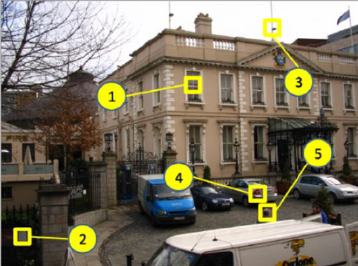
\includegraphics[width=0.5\textwidth]{passpoint.png}
		\caption{PassPoint.}
		\label{fig:PassPoint}
	\end{figure}
	%parte de hotspot
	Wiedenbeck en su investigación \cite{1}, asegura que las imágenes utilizadas en el sistema deben tener contenido significativo para el usuario, por lo que deben tener escenas concretas. Otro requisito es que la imagen seleccionada posea cientos de Hotspots diseminados de forma homogénea, de no ser así se reduciría el espacio de contraseñas y por ende aumentaría la vulnerabilidad ante diversos ataques, como los ataques de fuerza bruta y de diccionario.
	 
	Uno de los problemas que presenta este sistema es la improbabilidad de que el usuario seleccione en el momento de autenticación exactamente el mismo pixel de la fase de registro. Con la intención de erradicarlo surgen mecanismos de discretización, los cuales se encargan de establecer una tolerancia alrededor de cada punto. Sin embargo, esto disminuye el espacio de contraseñas y aumenta información relevante para llevar a cabo un ataque de diccionario. Un análisis sobre la relevancia del mecanismo de discretización en los sistemas de contraseñas gráficas se puede encontrar en \cite{14,15,16}. Por otro lado, en \cite{14,15,16,17} se describen los distintos métodos de discretización que se han desarrollado hasta ahora.

	%Una discusion acerca de la importancia del mecanismo de discretizacion en los esquemas de contrsaseñas graficas puede verse en [75,76,77 lisset], mientras que en [75,76,77,78 liset] pueden verse los diferentes metodos de discretizacion conocidos hasta el momento sad
	
	%modelo para hotspot
	En el trabajo \cite{18} se presenta un método que permite determinar si una imagen es adecuada para ser utilizada en esta técnica. Este método conduce al desarrollo de un modelo, diseñado para identificar las regiones de una imagen que los usuarios tienen mayor probabilidad de elegir como parte de sus contraseñas. Según sus experimentos, el modelo puede predecir puntos de interés (Hotspots) con una precisión de entre el 70 \% y el 80 \%, aunque el tamaño de la muestra utilizada es limitado. La aplicación de esta técnica en el sistema PassPoint sería especialmente útil para mejorar la confiabilidad en la asignación de imágenes. Por otro lado, en el estudio \cite{19} se demostró que incluso un pequeño cambio en la imagen puede influir en la elección de contraseñas por parte del usuario durante la fase de registro, afectando así su nivel de seguridad.   

	 

	%espacio de contrase;as osviel
	%En cuanto al espacio, segun (77 osviel) no se necesitarian muchos puntos para hacer la contraseña segura, con 5 o 6(en una imagen de 1024x725) se puede lograr mas que contraseñas que con 8 caracteres dentro del un alfebeto estandar de 64 letras. En la tabla (graphical vs alphanumeric) tomada de una investigacion se puede apreciar una comparacion entre los espacios de contraseñas graficas y alfanumericas variando el alfabeto , la longitud de la contraseña,tolerancia y tamaño de la imagen. Se puede apreciar que para 5 puntos y un tamaño de imgen razonable las contraseñas gráficas conservan un espacio de clave superior a las alfanumericas
	
	En relación al espacio de contraseñas, según \cite{1}, no sería necesario utilizar muchos puntos para crear una contraseña segura. Con solo 5 o 6 puntos (en una imagen de 1024x725), se podría lograr mayor seguridad que con contraseñas de 8 caracteres dentro de un alfabeto estándar de 64 símbolos. En la tabla \ref{tabla:comparar}, se muestra una comparación entre los espacios de contraseñas gráficas y alfanuméricas, considerando factores como el alfabeto, la longitud de la contraseña, la tolerancia y el tamaño de la imagen. Se observa que, con 5 puntos y un tamaño de imagen razonable, las contraseñas gráficas mantienen un espacio de clave superior al de las contraseñas alfanuméricas. Para resoluciones más actuales como 1366x768 (HD) o 1920x1080 (FHD) que son los estándares actuales, el espacio de claves  es mucho mayor al de las alfanuméricas, es decir, el espacio de claves mejora con la tecnología y no afecta la memorabilidad, cosa que no sucede con las alfanuméricas.
	
\begin{table}[h!]
	\centering
	\begin{tabular}{|c|c|c|c|c|c|}
		\hline
				 	 
		         		& Tamaño      &   Tamaño de &	Tamaño del  &Largo/No.  & Tamaño de \\ 
		                &   de imagen &  la cuadrícula    &  alfabeto/     & puntos de & espacio de \\ 
		                &             &      (píxeles)  & No.Cuadrículas & clic     & contraseñas \\\hline
		Alfanumérica    & N/A       & N/A     & 64   & 8  & 2.8x$10^{14}$  \\ \hline
		Alfanumérica    & N/A       & N/A     & 72   & 8  & 7.2x$10^{14}$ \\ \hline
		Alfanumérica    & N/A       & N/A     & 96   & 8  & 7.2x$10^{15}$\\ \hline
		Gráficas        & 451x331   & 20x20   & 373  & 5  &7.2x$10^{12}$\\ \hline
		Gráficas        & 1024x752  & 20x20   & 1925 & 5  &2.6x$10^{16}$\\ \hline
		Gráficas        & 1024x752  & 14x14   & 3928 & 5  &9.3x$10^{17}$\\ \hline
		Gráficas(1/2    & 1024x752  & 14x14   & 1964 & 5  & 2.9x$10^{16}$\\ 
		uso de la pantalla)   &   &    &  &  &  \\ \hline
	\end{tabular}
	\caption{Alfanuméricas vs Gráficas. Tomada de \cite{1}}
	\label{tabla:comparar}
\end{table}


	%tolerancia(discretizacion)
	

	
	
	
	%vantajas y desventajas
	
	%Gran n´umero de usuarios en las contrase˜nas gr´aficas tienden a seleccionar contrase˜nas que siguen determinados patrones, esto ayuda a la memorabilidad de las contrase˜nas pero al mismo tiempo contribuye a que sea relativamente f´acil encontrar un diccionario de ataque a este tipo de patrones. Como siguen cierto patr´on se les denomina contrase˜nas d´ebiles porque carecen de aleatoriedad. Ahora veremos cuales son los distintos patrones que tienden a seleccionar los usuarios a la hora de confeccionar sus contrase˜nas[3]

\section{Patrones DIAG y LINE}
%Además de la inclusión por parte de los usuarios de los Hotspots en las contraseñas, estas presentan otro tipo de debilidades como son los distintos tipos de patrones, leyes psicológicas o modelos de atención visual, los cuales son comúnmente utilizados por los usuarios para garantizar una mejor memorabilidad, lo que hace que sea más fácil contruir diccionarios de ataques estas contraseñas.


%Aparte de que los usuarios incluyen Hotspots en sus contraseñas
El problema de que los usuarios seleccionen imágenes que posean una cantidad reducida de Hotspots puede ser solucionado con un procesamiento previo de la misma, como se explica en la sección anterior, o brindando el sistema imágenes seguras. Sin embargo, existen debilidades que ocurren independientemente de la imagen empleada. Estas debilidades están relacionadas con el uso de patrones específicos, principios psicológicos o modelos de atención visual. Estos aspectos son habitualmente empleados por los usuarios con el fin de hacer que sus contraseñas sean más fáciles de recordar. Sin embargo, esta estrategia, aunque mejora la memorabilidad, también facilita la creación de diccionarios de ataque para descifrar las contraseñas. Los patrones, en unión con los Hotspots y las reglas perceptuales que los usuarios suelen seguir al elegir sus contraseñas, como la organización visual o la repetición de ciertas formas, hacen que estas sean vulnerables a distintos tipos  ataques.


%Algunos de los patrones reportados en  \cite{5,20,21,22,23,24,25} son: los patrones con una forma predeterminada(Z, W, V, C), los agrupados,  los regulares,y los patrones LOD y DIAG(o patrones diagonales) en los que se encuentran los patrones LINE(forma de línea).Los patrones DIAG y LINE se encuentran entre los que más tienden a seguir los usuarios, en \cite{20,21,22,23,24,25} caracterizan los patrones DIAG  por ser puntos que se encuentran formando arcos tanto horizontal como verticalmente y la suma de los valores absolutos de los ángulos es menor que 15\degree, en cambio los LINE se caracterizan por ser lineas horizontales y verticales que se definen como un subconjunto de los DIAG. 

En los estudios reportados en \cite{5,20,21,22,23,24,25}, se identificaron varios patrones comunes utilizados por los usuarios en la creación de contraseñas gráficas. Algunos de estos patrones incluyen formas predefinidas como Z, W, V, y C, patrones agrupados, regulares, y patrones LOD ( patrones que cumplen con la caracterización de que la distancia entre 2 puntos consecutivos es constante), además de los patrones DIAG y LINE, los cuales están relacionados con trayectorias diagonales o en línea. Entre estos, los patrones DIAG y LINE son los más frecuentemente utilizados por los usuarios según \cite{5}.

Los patrones DIAG se describen como configuraciones donde los puntos se organizan formando arcos en direcciones horizontales y verticales. Una característica distintiva de estos patrones es que la suma de los valores absolutos de los ángulos entre los puntos es menor a 15\degree. Por otro lado, los patrones LINE se caracterizan por ser líneas rectas, ya sean horizontales o verticales. Estos se consideran un subconjunto de los patrones DIAG, ya que ambas configuraciones comparten una estructura similar basada en la alineación de los puntos, pero los patrones LINE son más simples al ser exclusivamente rectos.

\begin{figure}[ht]
	\centering
	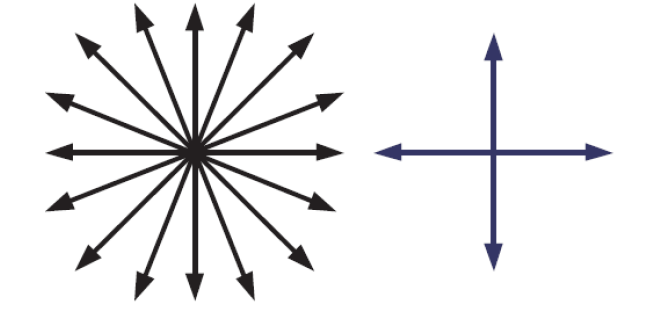
\includegraphics[width=0.5\textwidth]{DIAG_LINE.png}
	\caption{DIAG-LINE.}
	\label{fig:DIAG_LINE}
\end{figure}
 %\Van Oorschot,P.C...


%En \cite{21,22} tras realizar un estudio de 223 contraseñas gráficas en el escenario PassPoint seleccionadas por estudiantes en dos imágenes diferentes con un numero asequible de Hotspots distribuidos uniformemente en cada una de ellas, los autores consiguieron obtener del 48.2\% al 54.1\% de las mismas realizando un ataque de diccionario de 235.26 entradas utilizando patrones  DIAG y del 23.7\% al 52.3\% de dichas contraseñas realizando un ataque de 229.02 entradas utilizando  patrones LINE 

En un estudio realizado por los autores de \cite{21,22}, se investigaron 223 contraseñas gráficas en el sistema PassPoint. Estas contraseñas fueron seleccionadas por estudiantes que interactuaron con dos imágenes diferentes. Cada imagen contenía una cantidad manejable de Hotspots, distribuidos de manera uniforme entre ellas. Durante el experimento, los investigadores intentaron descifrar las contraseñas utilizando ataques de diccionario. Utilizando un diccionario de 235.26 entradas y patrones de tipo DIAG, los atacantes lograron obtener entre el 48.2\% y el 54.1\% de las contraseñas. Además, empleando un diccionario diferente de 229.02 entradas y patrones de tipo LINE, los resultados fueron algo menos efectivos, logrando recuperar entre un 23.7\% y un 52.3\% de las contraseñas. Estos resultados destacan la efectividad variable de los ataques de diccionario cuando se aplican a contraseñas gráficas en escenarios con patrones específicos.

%que me diga esto con otras palabras 
%toda la biblio de estas subsecciones son de  2018 scnc
%\subsection{Modelos de atención}
%Los Modelos Visuales De Atencion(MVA) estudian la forma en que las personas observan una imagen. Se estima que un grupo significativo de usuariios escoge los puntos siguiendo estos patrones (14). De esta manera se pueden construir dicccionarios con los grupos de puntos mas probables a seleccionar por el usuario.
%Los modelos computacionales de atencion Botton-Up, se definen normalmente por caracteristicas de las imagenes digitales tales como: la intensidad, el color y la orientacion(9,12). Por otra partelos modelos computacionales TopDown, pueden ser definidos por entrenamiento. La dificultad de estos ultimos se basa en que la tarea Top-down debe ser predefinida(ej.encontrar personas en una imagen) en um grupo de imagenes que se etiquetan con areas que contienen a los sujetos (14). Nos enfocaremos en la la propuesta de Itti(8,9) ya que exsite evidencia empírica  de que este captura la forma en que las persinas observan una imagen desde lo profundo hacia arriba(botton-up)(13). La idea principal de esta propuesta es que algunas areas de una imagen, son salientes o de alguna manera resaltan por que difieren del resto de su entorno. De esta manera dada una imagen  ek modelo devuelve las localizzaciones y el orden en que el ser humano de forma insconciente y automatica la observa. El proceso se compone de dos etapas. En la primera se crea un mapa de salientes basados en las caracteristicas visuales. En la segunda etapa se usa una red neuronal 'winner-take-wall' con el objetivo de replicar la forma en que el usuario observaria la imagen. En(15) se desarrolla un ataque automatico de diccionario que se basaba solo en variaciones de la primera etapa donde utilizaba deteccion de esquinas para encontrar puntos referenciables, luego en (14) se describe como seria la segunda etapa del proceso.
%La idea principal ( primera etapa ) de esto metodo sirve de soporte para las tecnocas de analisis y procesamiento de imagenes. Estas se vasen en la deteccion de esquinas y centroides asi como la plicacion de herramientas y algoritmos de inteligencia artificial para detectar objetos en imagenes

\section{Triangulaciones de Delaunay}
\textbf{Definición(Triángulación de Delaunay):} Una triangulación del conjunto $P=\{p_1,p_2 ... p_n\}$ de los puntos sobre el plano es de Delaunay, si y solo si la circunferencia circunscrita de cualquier triángulo en la red no contiene un punto $p_i$ en su interior. Como ejemplos de esta están las figuras \ref{cumple}, \ref{no_cumple} y  \ref{Triangulación}. Esta definición es conocida como condición de Delaunay \cite{26,27,28}.\\    

		{\large{\textbf{Propiedades elementales de las triangulaciones de Delaunay}}}\\

	Una triangulación de Delaunay presenta las siguientes tres propiedades elementales:
	
	\begin{enumerate}
		\item La frontera externa de la triangulación de Delaunay forma la envoltura convexa del conjunto de puntos.
		\item El ángulo mínimo dentro de todos los triángulos de Delaunay esta maximizado, es decir, se evita obtener resultados con ángulos demasiados agudos. Como consecuencia de lo anterior, los triángulos generados en una triangulación tienden a ser lo más equilátero posible. Esto  es debido a que todo triángulo no equilátero siempre tiene algún ángulo menor que 60{\degree }.
		\item La triangulación es única cuando ningún borde de la circunferencia circunscrita contiene más de tres vértices de la red. 
	
	\end{enumerate}
		

	
	\begin{figure}[h]
		\centering
		\begin{minipage}{0.45\textwidth}
			\centering
			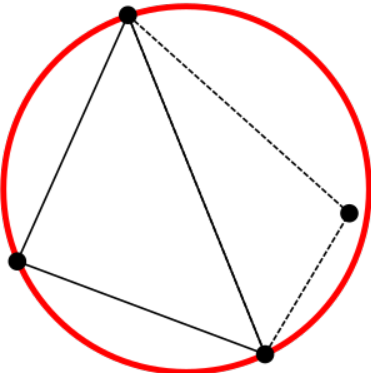
\includegraphics[width=0.44\linewidth]{no_td.png}  % Inserta la primera imagen
			\caption{Esta triangulación no cumple condición de Delaunay}
			\label{no_cumple}
			
		\end{minipage}\hfill
		\begin{minipage}{0.45\textwidth}
			\centering
			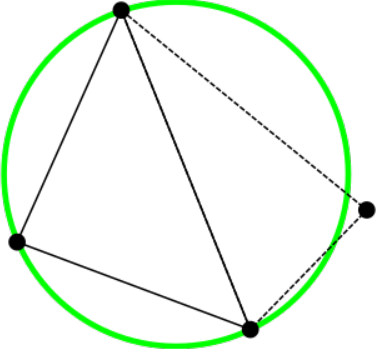
\includegraphics[width=0.5\linewidth]{si_td.png}  % Inserta la segunda imagen
			\caption{Esta triangulación sí cumple condición de Delaunay}
			\label{cumple}
		\end{minipage}
	\end{figure}

	
	Un aspecto clave al trabajar con triangulaciones de Delaunay es determinar si una triangulación es válida. Para lograr esto, se recurre a la fórmula de Euler, que es una herramienta fundamental en geometría computacional. Considerando un conjunto de puntos \textit{P} de \textit{n} elementos, si hay una cantidad \textit{h} de puntos que pertenecen a la envoltura convexa de dicho conjunto, la fórmula permite calcular ciertas propiedades de la triangulación. Según esta, la triangulación de Delaunay resultante tendrá un total de 2\textit{n}-2-\textit{h} triángulos y 3\textit{n}-3-\textit{h} aristas \cite{29}. Notemos que para  5 puntos de una contraseña, como máximo podemos obtener 5 triángulos de Delaunay pues \textit{n}=5 y \textit{h} puede variar entre 3, 4 o 5.
	
	\begin{figure}[ht]
		\centering
		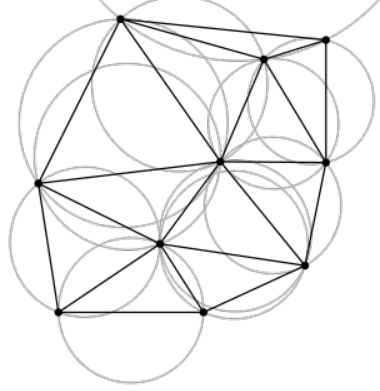
\includegraphics[width=0.3\textwidth]{td_10pts.png}
		\caption{Triangulación de Delaunay para 10 puntos}
		\label{Triangulación}
	\end{figure}

\section{Antecedentes en la detección de patrones DIAG y LINE o patrones suaves}	
	En el contexto de la seguridad informática, la detección de patrones en contraseñas gráficas ha emergido como un aspecto crucial para garantizar la robustez de los sistemas de autenticación, especialmente en entornos como PassPoint. La identificación y evaluación de patrones específicos, como los patrones DIAG y LINE, se ha vuelto fundamental para mitigar vulnerabilidades y fortalecer la seguridad en estos sistemas.
	
	Los estudios previos han destacado la efectividad de diversos métodos en la detección de contraseñas débiles que siguen patrones suaves. En particular, dos enfoques sobresalen en esta área: el algoritmo diseñado para detectar contraseñas con patrones suaves en PassPoint \cite{3} y el \textit{test} basado en el promedio de los ángulos máximos de los triángulos de Delaunay \cite{13} para la identificación de patrones DIAG y LINE en contraseñas gráficas.
	
	En esta sección, se analizarán en detalle estos dos enfoques, centrándose en su eficacia, metodología y resultados. El objetivo es comprender cómo estos métodos contribuyen a la detección y evaluación de contraseñas débiles que siguen patrones predefinidos, así como su relevancia en la mejora de la seguridad en sistemas de autenticación gráfica como PassPoint.

\subsection{Algoritmo para la detección de contraseñas con patrones suaves en PassPoint}

%En \cite{3} se propuso un algoritmo para la detección de contraseñas con patrones suaves en PassPoint. El algoritmo propuesto recibe como entrada los puntos seleccionados por el usuario en la contraseña y un parámetro   $D(\varphi\degree)$  que es un valor de tolerancia. Con los 5 puntos dados de la contraseña se calculan los tres ángulos entre los segmentos consecutivos formados por los puntos, el algoritmo detecta que está ante la presencia de una contraseña con un patrón suave cuando los tres ángulos son mayores que $D(\varphi\degree)$.
En \cite{3}, Rodriguez presentó un algoritmo diseñado para identificar contraseñas con patrones suaves en el método PassPoint. Este algoritmo toma como datos de entrada los puntos seleccionados por el usuario al crear su contraseña, junto con un parámetro de tolerancia, representado como $D(\varphi\degree)$. A partir de los 5 puntos que componen la contraseña, se calculan los tres ángulos formados entre los segmentos consecutivos que conectan dichos puntos. El algoritmo determina que una contraseña presenta un patrón suave cuando los tres ángulos calculados superan el valor del parámetro $D(\varphi\degree)$.

La cuestión de este algoritmo radica en la selección del valor $D(\varphi\degree)$, pues este es el mayor determinante en la decisión del mismo. Para la solución de este problema se realizó una implementación básica del PassPoint para la web con dos imágenes de 700x400. A partir de ello, un grupo de 60 alumnos de la Universidad de Ciencias Informáticas crearon 397 contraseñas, las cuales se clasificaron visualmente y se decidió que 124 de ellas cumplían con el patrón de suavidad. 

En un primer experimento se aplicó el algoritmo propuesto a las 124 contraseñas variando con paso 10 el parámetro $D(\varphi\degree)$, y de esta manera se determinaron los falsos negativos obtenidos por el algoritmo para cada valor de $D(\varphi\degree)\in$ \{20,30,40,50....,150\}. Se observó que al aumentar $D(\varphi\degree)$ se reducen los falsos negativos, y que para valores de $D(\varphi\degree)$ mayores a $80\degree$  ocurre poca variación en la cantidad de contraseñas detectadas. Incluso para $D(\varphi\degree)=150\degree$ quedaron aún 3 contraseñas sin ser detectadas, comentando el autor de dicho algoritmo en [3] que el error podría ser debido a la clasificación del observador.  

En un segundo experimento se aplicó el algoritmo para las 397 contraseñas registradas inicialmente por los 60 usuarios y los mismos valores de $D(\varphi\degree)$ que en el experimento anterior, para identificar cuántas nuevas contraseñas detectaba el algoritmo que no estaban en la clasificación inicial. Se pudo apreciar que el número crece a partir de que $D(\varphi\degree)$ es mayor que 50\degree. Dada la contradicción entre las contraseñas detectadas por el algoritmo y las clasificadas por el observador, se realizó un análisis de las contraseñas no clasificadas por este pero sí por el algoritmo y se pudo demostrar que sí cumplían con el patrón de suavidad. Esto sugirió que el observador pudo haber cometido errores en la clasificación, ya que el usuario que eligió la contraseña intentaba establecer conexiones entre los puntos, aunque la suavidad de estas relaciones no sea evidente para quien observa.
 

Como tercer experimento el algoritmo fue aplicado sobre un conjunto de 400 contraseñas aleatorias para detectar los falsos positivos para cada valor de $D(\varphi\degree)$. Según los resultados, se sugirió usar por defecto $D(\varphi\degree)$=130\degree, ya que establecía un buen equilibrio entre falsos positivos y falsos negativos. La figura \ref{frecuencia}  extraída de \cite{3} proporciona la información necesaria para ajustar este parámetro según las necesidades del usuario. Según \cite{3}, incrementar $D(\varphi\degree)$ mejora la seguridad, mientras que reducirlo favorece la usabilidad del sistema.

\begin{figure}[ht]
	\centering
	\includegraphics[width=1\textwidth]{grafosviel.png}
	\caption{Frecuencia de falsos positivos vs falsos negativos según ${D(\varphi\degree)}$.} Tomada de \cite{3}.
	\label{frecuencia}
\end{figure}

A partir de los resultados de cada experimento, Rodriguez afirmó que se obtuvo un criterio efectivo para detectar la existencia de patrones de suavidad en las contraseñas de la técnica de autenticación gráfica PassPoint en imágenes de 700x400 píxeles. En \cite{3} se puede observar el algoritmo propuesto así como una implementación del mismo en Python. Además el algoritmo permitió constatar que en muchas ocasiones el usuario crea una dependencia entre los puntos que no se nota a simple vista por un observador, sin embargo puede ser detectada por el algoritmo con parámetro de tolerancia variable.


\subsection{\textit{Test} de detección de patrones DIAG y LINE en el sistema PassPoint basado en los ángulos máximos de los triángulos de Delaunay  }


%En \cite{13} se propuso un novedoso test para detectar  contraseñas gráficas en PassPoint que sigan patrones DIAG y LINE, valido para todos los tamaños de imágenes con ratio 16:9.

%Para la construcción de este test, se formuló y se probó como hipótesis inicial que la media de los ángulos máximos de los triángulos de la triangulación de Delaunay de los cinco puntos de una contraseña gráfica en PassPoint es un estadístico eficaz para evaluar y decidir si la contraseña seleccionada por el usuario sigue o no un patrón DIAG o LINE. Los experimentos mostraron que las contraseñas que siguen patrones DIAG o LINE tenían una media del estadígrafo superior a la media estimada para las contraseñas con puntos seleccionados aleatoriamente. Se comprobo que  el estadístico seleccionado distribuye con normalidad, por lo que se construye un test de una cola(derecha) para media de una distribución Normal, que evalúa la hipótesis nula de que la contraseña no sigue un patrón DIAG o LINE frente a la alternativa de que sigue un patron DIAG o LINE.

%La eficacia de la prueba propuesta se evaluó en seis bases de datos de 10000 contraseñas cada una, tres de estas con contraseñas que forman patrones DIAG y tres con LINE, para cada patrón las bases de datos se dividieron según los ángulos entre los segmentos consecutivos lo cual se determina en \cite{5} como una frecuencia mayor a la media. 
%La prueba logró detectar el 100\% de las contraseñas gráficas analizadas que siguen patrones DIAG y LINE cuyos segmentos consecutivos tienen una amplitud máxima entre 180\degree y 150\degree(Db1.DIAG, Db2.DIAG, Db1.LINE, Db1.LINE), para los cinco niveles de significación. Para los patrones con una amplitud  entre 150\degree y 145\degree (Db3.DIAG, Db3.LINE), en el caso de los niveles de significación $\alpha$=0.2 y $\alpha$=0.1 logró detectar el 100\% de las contraseñas , mientras que para $\alpha$ $\in$ \{0.05, 0.02, 0.01\} la eficacia fue aproximadamente del 88\%, 42\% y 16\% respectivamente. Para fines generales los autores recomiendan como nivel de significación {$\alpha$=0.05} pues proporciona unos valores de detección superiores al 91\%  para patrones DIAG y 88\% para patrones LINE.\\ 

%%%%%%%%%%%%%%%%%%%%%%%%%%%%%%%%%%%%%%%%%%%%%%

En \cite{13} se propuso un innovador \textit{test} para la detección de contraseñas gráficas débiles en el sistema PassPoint, diseñado específicamente para identificar contraseñas que sigan patrones de tipo DIAG y LINE. Este \textit{test} se aplica de manera efectiva a imágenes con una relación de aspecto 16:9, válida para una amplia gama de tamaños de imagen. Para la construcción de este \textit{test}, se desarrolló y probó una hipótesis inicial en la que se utilizó como estadígrafo la media de los ángulos máximos de los triángulos resultantes de la triangulación de Delaunay en los cinco puntos de una contraseña gráfica en PassPoint. Este enfoque demostró ser un método eficaz para evaluar y determinar si la contraseña seleccionada sigue un patrón DIAG o LINE.

Los resultados experimentales revelaron que las contraseñas que se ajustan a estos patrones tenían una media del estadígrafo significativamente más alta que aquellas generadas de forma aleatoria. Además, se comprobó que el estadígrafo utilizado seguía una distribución normal, lo que permitió desarrollar un \textit{test} de una cola (derecha) basado en la media de una distribución normal. Este \textit{test} evalúa la hipótesis nula, que afirma que la contraseña no sigue un patrón DIAG o LINE, frente a la alternativa de que sí sigue uno de estos patrones.

La eficacia del \textit{test} se evaluó utilizando seis bases de datos que contenían 10 000 contraseñas cada una. Tres de estas bases incluían contraseñas que formaban patrones DIAG y tres contenían patrones LINE, y a su vez cada una con distintos niveles de suavidad. Las bases de datos fueron segmentadas según los ángulos entre los segmentos consecutivos, una frecuencia que se determinó en \cite{5} como mayor a la media. El \textit{test} logró detectar el 100\% de las contraseñas gráficas que seguían los patrones DIAG y LINE, para segmentos consecutivos con una amplitud máxima entre 150° y 180° (Db1.DIAG, Db2.DIAG, Db1.LINE, Db2.LINE) en todos los niveles de significación evaluados.

Para contraseñas cuyos patrones tenían una amplitud entre 135° y 150° (Db3.DIAG, Db3.LINE), el \textit{test} logró una detección del 100\% en los niveles de significación $\alpha$ = 0.2 y $\alpha$ = 0.1. Sin embargo, en los niveles de significación más bajos  $\alpha$ $\in$ \{0.05, 0.02, 0.01\}, la tasa de detección disminuyó a aproximadamente 88\%, 42\% y 16\%, respectivamente. Para fines generales, los autores recomendaron  utilizar un nivel de significación de $\alpha$ = 0.05, ya que este valor ofrece resultados superiores al 91\% de detección para patrones DIAG y 88\% para patrones LINE, a cambio de solo un falso positivo cada 20.



%%%%%%%%%%%%%%%%%%%%%%%%%%%%%%%%%%%%%%
%En el estudio mencionado en la referencia [13], se propuso un test innovador destinado a detectar contraseñas gráficas en PassPoint que siguieran los patrones DIAG o LINE, siendo este método válido para imágenes de cualquier tamaño con una relación de aspecto de 16:9. Para desarrollar este test, se planteó inicialmente y se sometió a prueba la hipótesis de que la media de los ángulos máximos de los triángulos en la triangulación de Delaunay de los cinco puntos clave de una contraseña gráfica en PassPoint podría ser un indicador efectivo para determinar si la contraseña elegida por el usuario seguía o no un patrón DIAG o LINE.

%Los resultados experimentales revelaron que las contraseñas que cumplían con los patrones DIAG o LINE presentaban un promedio del estadígrafo superior al promedio estimado para aquellas contraseñas cuyos puntos habían sido seleccionados aleatoriamente. Se confirmó que el estadístico seleccionado seguía una distribución normal, lo que permitió la construcción de un test unidireccional (hacia la derecha) para la media de una distribución normal. Este test evaluaba la hipótesis nula de que la contraseña no seguía un patrón DIAG o LINE en contraposición a la hipótesis alternativa de que sí lo seguía.

%La efectividad de esta prueba fue evaluada en seis bases de datos, cada una conteniendo 10,000 contraseñas. Tres de estas bases de datos consistían en contraseñas que formaban patrones DIAG y las otras tres en patrones LINE. Para cada patrón, las bases de datos se dividieron según los ángulos entre los segmentos consecutivos, determinando que una frecuencia mayor a la media, según Chiasson, indicaba la presencia del patrón. El test logró detectar el 100% de las contraseñas gráficas analizadas que seguían los patrones DIAG y LINE, cuyos segmentos consecutivos tenían una amplitud máxima entre 180° y 150°.

%En el caso de los patrones con una amplitud entre 150° y 145°, el test logró detectar el 100\% de las contraseñas para los niveles de significación α=0.2 y α=0.1, mientras que para α ∈ {0.05, 0.02, 0.01}, la eficacia fue aproximadamente del 88%, 42% y 16% respectivamente. En términos generales, los autores recomendaron un nivel de significación de α=0.05, ya que proporcionaba valores de detección superiores al 91% para patrones DIAG y 88% para patrones LINE.


\setcounter{chapter}{2}

\chapter*{\LARGE{Capítulo 2}}
\addcontentsline{toc}{chapter}{2. Detección de patrones DIAG y LINE en PassPoint, basado en el promedio de los ángulos máximos de los triángulos de Delaunay, condicionado al número de triángulos}

\vspace{-2em} % Reduce el espacio entre el título y el texto siguiente

\noindent\textbf{\LARGE Detección de patrones DIAG y LINE en PassPoint, basado en el promedio de los ángulos máximos de los triángulos de Delaunay, condicionado al número de triángulos}\\
\vspace{2em}
\\	
En \cite{13} se demostró que el promedio de los ángulos máximos de los triángulos de Delaunay es un estadígrafo eficaz para la detección de patrones DIAG y LINE. Teniendo en cuenta que las contraseñas en PassPoint se crean con la selección de 5 puntos, los posibles números de triángulos de Delaunay pueden ser 3, 4 o 5 como se mostró en la sección 1.3. En las próximas secciones se proponen tres \textit{test} de detección de contraseñas  que siguen patrones DIAG o LINE en PassPoint, basados en el promedio de los ángulos  máximos de los triángulos de Delaunay, pero  realizando un análisis separado por cada número de triángulos en su triangulación.
En cada subsección se determinarán las distribuciones a las qué se ajustaron los promedios de los ángulos máximos de los triángulos de Delaunay para el número de triángulos correspondiente, a través  del software EasyFit 5.6. A partir de ello se construirá un \textit{test} estidístico para la detección de contraseñas con patrones DIAG y LINE, y se evaluará su efectividad estimando los errores de  tipo I y de tipo II cometidos.

La justificación del uso de EasyFit 5.6 para ajustar los datos a una distribución conocida se basa en que esta versión del software contiene un total de 54 distribuciones conocidas y una implementación de los \textit{test} de bondad de ajuste Kolmogorov-Smirnov, Anderson-Darling y Chi-Cuadrado, que son empleados para encontrar la distribución que mejor se ajuste a los datos.


\setcounter{section}{0}
\section{Contraseñas con 3 triángulos en su triangulación de Delaunay }
En esta sección cuando se hace referencia  al promedio de los ángulos máximos de los triángulos de Delaunay  de las contraseñas gráficas en PassPoint, nos referiremos a las contraseñas que posean 3 triángulos en su triangulación de Delaunay, figura \ref{3TD}.
\newpage
	\begin{figure}[ht]
	\centering
	
	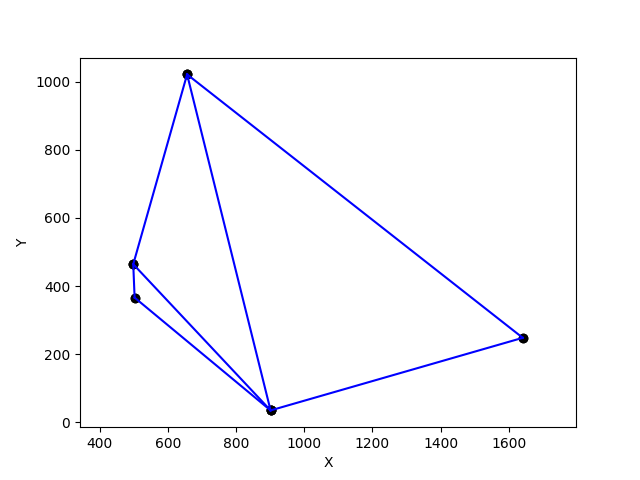
\includegraphics[width=0.41\textwidth]{alea3td.png}
	\caption{Contraseña gráfica de 5 puntos con una triangulación de Delaunay de 3 triángulos.}
	\label{3TD}
\end{figure}
\subsection{Media muestral, desviación estándar y distribución del promedio de los ángulos máximos de los triángulos de Delaunay }
	\textbf{Diseño del experimento \#1.1}.
	
	 Para estimar la media muestral, desviación estándar y distribución del promedio de los ángulos máximos de los triángulos de Delaunay para contraseñas gráficas en PassPoint, se generaron aleatoriamente 1000 contraseñas gráficas de 5 puntos en una imagen de 1920x1080. Para cada una de estas contraseñas se  construyó  su correspondiente triangulación  de Delaunay  y se  determinó el promedio  de los ángulos máximos de su triangulación de Delaunay resultante. A la base de datos que contiene los 1000 promedios se le denominó BD.1. Una vez creada dicha base de datos, se utilizó el software EasyFit 5.6 para ajustar dichos datos a una distribución conocida, además de conocer la media y la desviación estándar.
	 
	 \textbf{Resultados del experimento \#1.1.}
	 
	 Los resultados obtenidos indican que los datos poseen una media de $99.178\degree$ y una desviación estándar de $15.751\degree$.
	 En la tabla \ref{teo_BD1}  se muestran las 6 distribuciones a las que más se ajustaron a los datos encontrados en BD.1, teniendo en cuenta los tres test de bondad de ajuste mencionados anteriormente. Encontrándose en el primer lugar \textit{Johnson SB} con los parámetros $\gamma=1.9152$, $\delta=1.4296$, $\lambda134.77$ y $\xi=68.377$.  Sin embargo, cabe destacar que los datos se ajustaron a  distribuciones conocidas, sin encontrarse entre ellas la distribución Normal, al contrario de como se esperaba, pues se rechazan para esta distribución los tres test de bondad de ajuste aplicados para todos los niveles de significación, como muestra la tabla \ref{teo_BD1}, además que la misma ocupa el puesto 34. En la figura \ref{3TD_BONDAD} se  muestran los resultados de tres de los \textit{test} de bondad de ajuste aplicados a la distribución \textit{Johnson SB} sobre  datos contenidos en BD.1 donde  para ninguno de los tres test de bondad de ajuste  se rechaza la hipótesis nula de que los datos provienen de la distribución teórica \textit{Johnson SB}, aceptandolos para todo nivel de significación  y por tanto indicando un buen ajuste. En la figura \ref{3TD_FDP}  se muestra la función de densidad de probabilidad de la misma.
	  	\begin{figure}[ht]
	  	\centering
	  	
 	  	\includegraphics[width=0.6\textwidth]{3td_BONDAD.png}
	  	\caption{\textit{Test} de bondad de ajuste aplicados a la distribución \textit{Johnson SB} sobre BD.1.}
	  	\label{3TD_BONDAD}
	  \end{figure}
	  
	  
	 
	 A partir de este resultado, en el resto de la sección se asume que la muestra BD.1 y, por tanto, el promedio de los ángulos máximos de las triangulaciones de Delaunay que tengan tres triángulos en las contraseñas de PassPoint, proceden de una distribución \textit{Johnson SB}. Por lo que se puede asumir que las contraseñas que incumplan esta propiedad no son aleatorias.
	 La aplicación práctica de este criterio se facilita porque después de  aplicar la transformación de \textit{Johnson SB}  mediante la fórmula \cite{30} :
	 
	  
	 \[
	 P_D^{N} = J_{SB}(P_D) = \gamma + \delta \times ln\left(\frac{P_D - \xi}{\lambda + \xi - P_D}\right),
	 \]
	 con los parámetros correspondientes, el promedio transformado debe seguir una distribución normal estándar $P_D^{N}\sim N(0,1)$. Basado en la propiedad anterior, la detección de la no aleatoriedad de las contraseñas se reduce a aplicar un \textit{test} de media para la distribución normal del estadígrafo muestral transformado a \textit{Johnson SB}.
	 \begin{figure}[ht]
	 	\centering
	 	
	 	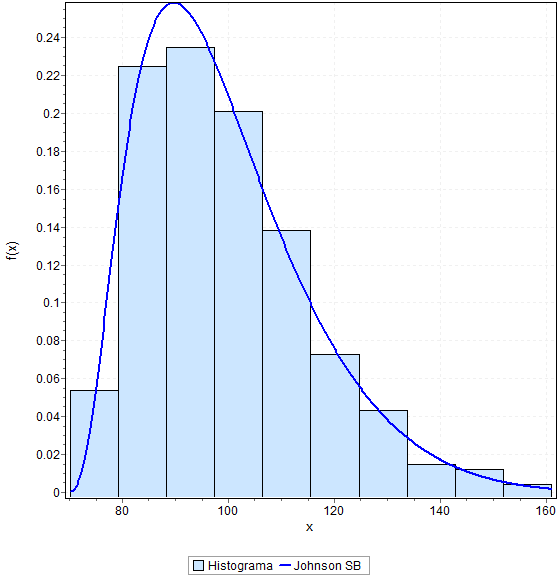
\includegraphics[width=0.5\textwidth]{3td_fdp.png}
	 	\caption{Función de densidad de probabilidad de la  distribución \textit{Johnson SB} para BD.1.}
	 	\label{3TD_FDP}
	 \end{figure}
	 
	 
\subsection{\textit{Test} basado en el promedio de los ángulos máximos de triangulaciones de Delaunay con tres triángulos, para la detección de patrones DIAG y LINE en las contraseñas de PassPoint}
Dado  que el promedio de los ángulos máximos de los triángulos de Delaunay distribuye \textit{Johnson SB}, se propone un  \textit{test} estadístico para identificar contraseñas con patrones DIAG y LINE en PassPoint. La propuesta consiste en un \textit{test} de una cola (derecha) basado en el promedio de los ángulos máximos de los triángulos de Delaunay transformados a una distribución normal estándar mediante la transformación \textit{Johnson SB}.
Este se enfoca en la amplitud de los ángulos en lugar de las dimensiones de los lados o cualquier otra característica que pueda cambiar con el tamaño de la imagen. Por lo tanto, será aplicable a todas las imágenes con una relación de aspecto de 16:9. En estas imágenes, las dimensiones serán proporcionales y los triángulos dentro de ellas también serán proporcionales, lo que permite formalizar la \textit{test} propuesta de la siguiente manera:

\begin{enumerate}
	\item Variable aleatoria X: promedio de los ángulos máximos de los triángulos de Delaunay de contraseñas de 5 puntos con 3 triángulos en su triangulación.
	\item Estadígrafo: \[
	Z= J_{SB}(X) =  \gamma + \delta \times ln\left(\frac{X - \xi}{\lambda + \xi - X}\right)
	\]

	\item Hipótesis nula: \[H_0:E(Z)=0\]
	\begin{itemize}
		\item La contraseña gráfica seleccionada por el usuario es aleatoria si el promedio de los ángulos máximos de los triángulos de Delaunay  transformados mediante la fórmula de \textit{Johnson SB} a una normal estándar es igual a 0.
	\end{itemize}
	
	
	\item Hipótesis alternativa: \[H_a:E(Z)>0\]
			\begin{itemize}
			\item La contraseña gráfica seleccionada por el usuario posee patrones DIAG o LINE  si el promedio de los ángulos máximos de los triángulos de Delaunay  transformado mediante la fórmula de \textit{Johnson SB} a una normal estándar es mayor a 0.
		\end{itemize}
	
	\item  Región de Rechazo: $\{z$:$Z>z_\alpha\}$, donde $\alpha$ es el nivel de significación establecido por el usuario. 
	
	\item Criterio de decisión:
	\begin{itemize}
		\item Para los cinco niveles de significación establecidos, se decide que la contraseña gráfica seleccionada por el usuario no sigue un patrón aleatorio si al transformar el promedio de los ángulos máximos de los triángulos de Delaunay mediante la transformación \textit{Johnson SB}, el valor obtenido pertenece a la región crítica. 
	\end{itemize}
	\end{enumerate}	 

\subsection{Implementación del \textit{Test} propuesto:}
Para la implementación del \textit{test} propuesto, se toman las coordenadas \((x_i, y_i)\) de cada uno de los \(p_i\) puntos, \(i = 1, \ldots, 5\) como valores de entrada. A partir de estos puntos, se construye la triangulación Delaunay utilizando la función \textit{Delaunay} de scipy.spatial.

Luego, la longitud de los lados de cada triángulo se determina por la distancia euclidiana de dos a dos de los puntos que lo forman, de la siguiente ecuación:

\[
a = \sqrt{(x_{1} - x_{2})^2 + (y_{1} - y_{2})^2} .
\]

Para encontrar los ángulos de cada triángulo, se aplica la Ley de los Cosenos:

\[
\theta = \arccos\left(\frac{c^2 + a^2 - b^2}{2ab}\right), \quad \phi = \arccos\left(\frac{a^2 + b^2 - c^2}{2ab}\right), \quad \psi = \arccos\left(\frac{b^2 + c^2 - a^2}{2bc}\right).
\]

Es necesario encontrar el máximo de estos tres ángulos \(\theta\), \(\phi\), y \(\psi\). Es análogo para los triángulos restantes de la triangulación Delaunay. Una vez que se hayan obtenido los ángulos máximos de la triangulación Delaunay, se calcula su promedio, con el cual se obtiene el valor de  \(X\). La hipótesis nula se rechaza dependiendo de si la estadística \(Z\) pertenece a la región de rechazo para el \(\alpha\) establecido.

Una posible implementación de esta prueba en Python sería:
\begin{itemize}
	\item points: 5 puntos de la contraseña. 
	\item gamma, delta, lambd, xi: parámetros correspondientes a la distribución \textit{Johnson SB} obtenida.
	\item rg: límite inferior de la región de rechazo según el nivel de significación escogido.
	
\end{itemize}
La implementación del \textit{test} retorna 0 cuando se rechaza la hipótesis nula y 1 en caso contrario



\begin{lstlisting}
	def test(points,gamma,delta,lambd,xi,rg):
		triangulation=Delaunay(points)
		angles=[]
		for i in triangulation:
			a=distancia_puntos(points[i[0]],points[i[1]])
			b=distancia_puntos(points[i[1]],points[i[2]])
			b=distancia_puntos(points[i[2]],points[i[0]])
			angles.append(angle_max(a,b,c))
		X=mean(angles)
		Z=gamma + delta * np.log((x - xi) / (lambd - x + xi))
		if Z>rg:
		return 0
		else:
		return 1
	
	def distancia_puntos(punto1, punto2):
		return math.sqrt((punto1[0] - punto2[0])**2 +
		(punto1[1] - punto2[1])**2)
	
	def angle_max(distancia_ab, distancia_bc, distancia_ca):
		angulo_A = math.degrees(math.acos(
		(distancia_bc**2 + distancia_ca**2 - distancia_ab**2) 
		/ (2 * distancia_bc * distancia_ca)
		))
		angulo_B = math.degrees(math.acos(
		(distancia_ca**2 + distancia_ab**2 - distancia_bc**2) 
		/ (2 * distancia_ca * distancia_ab)
		))
		angulo_C = 180 - angulo_A - angulo_B  
		return max(angulo_A, angulo_B, angulo_C)
\end{lstlisting}

En cuanto a la complejidad, las funciones \textit{distancia\_puntos} y \textit{angle\_max} solo poseen operaciones elementales, por lo que su complejidad es \textit{O(1)}. La función test en su primera línea hace un llamado a la función  \textit{Delaunay} (línea 2) de \textit{scipy.spatial}, esta posee una complejidad de \textit{O(N logN)} debido a que el algoritmo subyacente utilizado por \textit{Scipy} es el algoritmo de \textit{Qhull}. Seguido en el algoritmo se itera por la triangulación obtenida (líneas 4-8), la cual poseen como máximo \textit{n} triángulos , dentro de cada iteración se hacen llamados a las  funciones \textit{distancia\_puntos} y \textit{angle\_max}  que son \textit{O(1)}, por tanto el costo del iterador es \textit{O(N)}. Las operaciones restantes son \textit{O(1)} (líneas 9-14), por tanto el costo total sería \textit{O(1)}+\textit{O(N)}+\textit{O(N logN)}=\textit{O(N logN)} por ley de la suma.
\subsection{Validación del \textit{test} propuesto}
	
	Con el objetivo de validar la eficacia del \textit{test} se realizó una estimación de la probabilidad de cometer errores de tipo I (falsos positivos) y de tipo II (falsos negativos).
		 
	\textbf{Diseño del experimento \#1.2 : Estimación de la probabilidad de cometer un error de tipo I} 
	
	Para estimar la probabilidad de que la prueba decida que la contraseña gráfica contiene un patrón DIAG o LINE cuando, en verdad, sigue un patrón aleatorio (error de tipo I o falsos positivos), se generó una base de datos BD.1.RANDOM con 10 000 contraseñas gráficas aleatorias sobre la imagen. El \textit{test} descrito en la sección 2.1.3 se aplicó a cada una de estas contraseñas gráficas para los valores de $z_\alpha \in \{$0.842, 1.282, 1.645, 2.054, 2.326$\}$ correspondientes a los niveles de significación $\alpha \in \{$0.2, 0.1, 0.05, 0.02, 0.01$\}$.
	


\textbf{Resultados del experimento \#1.2}

Las probabilidades estimadas de cometer un error de tipo I ($\hat{\alpha}$) mediante el \textit{test} son ligeramente superiores  a las probabilidades teóricas preestablecidas ($\alpha$), véase en la figura \ref{Teorico vs Observado} y en la tabla \ref{3td:error1-prob}. Por tanto, se puede concluir que el criterio de decisión propuesto es válido.
	\begin{figure}[ht]
	\centering
	
	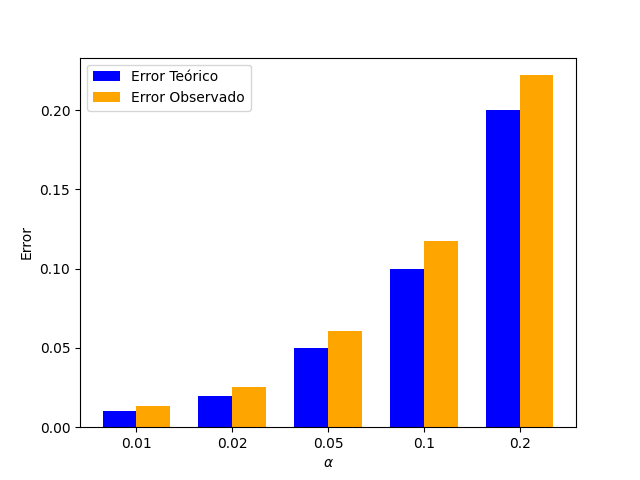
\includegraphics[width=0.8\textwidth]{3td_teo_obs.png}
	\caption{Comparación entre las probabilidades teóricas ($\alpha$) y estimadas ($\hat{\alpha}$) de cometer un error de tipo I. }
	\label{Teorico vs Observado}
\end{figure}\\
\begin{table}[h!]
	\centering
	\begin{tabular}{|c|ccccc|}
		\hline
		$\alpha$ &  0.2 &  0.1 &  0.05 & 0.02 &  0.01 \\
		\hline
		$\hat{\alpha}$ & 0.2221 & 0.1178 & 0.0605 & 0.0251 & 0.0132 \\
		\hline
		RC $H_0$ &  $Z>$0.842& $Z>$1.282& $Z>$1.645& $Z>$2.054& $Z>$2.326 \\
		\hline
	\end{tabular}
	\caption{Estimación de la probabilidad ($\hat{\alpha}$) del error de tipo I derivado de la prueba.}
	\label{3td:error1-prob}
\end{table}
\\
\textbf{Experimento \#1.3: Estimación de la probabilidad de cometer un error de tipo II}

Para estimar la probabilidad $\hat{\beta}$ de que el \textit{test} detecte una contraseña gráfica como aleatoria cuando sigue un patrón DIAG o LINE  (error tipo II o falsos negativos), se crearon 3 bases de datos, que en conjunto contienen 30 000 contraseñas gráficas de 5 puntos que siguen patrones DIAG y LINE:
\begin{itemize}
	\item BD.DIAG\_LINE.1.3.1: 10 000 contraseñas gráficas que siguen patrones DIAG o LINE con una anchura máxima entre dos segmentos consecutivos de 15\degree. Base de datos con mayor nivel de suavidad. 
	\item BD.DIAG\_LINE.1.3.2: 10 000 contraseñas gráficas que siguen patrones DIAG o LINE con una anchura máxima entre dos segmentos consecutivos que varia entre $15\degree$ y $30\degree$. Base de datos medianamente suave.
	\item BD.DIAG\_LINE.1.3.3: 10 000 contraseñas gráficas que siguen patrones DIAG o LINE con una anchura máxima entre dos segmentos consecutivos que varia entre $30\degree$ y $45\degree$. Base de datos con menor nivel de suavidad.
\end{itemize}
\textbf{Resultados del experimento \#1.3}

Los resultados obtenidos por el \textit{test}  para cada una de las bases de datos y los  niveles de significación preestablecidos se muestran en la tabla. \ref{tab:error2-prob}

\begin{table}[h!]
	\centering
	\begin{tabular}{|c|ccc|}
		\hline
		 $\alpha$& BD.DIAG\_LINE.1.3.1 & BD.DIAG\_LINE.1.3.2 & BD.DIAG\_LINE.1.3.3  \\
		\hline
		0.2 & 0     & 0          & 0.0571     \\
		0.1 & 0     & 0          & 0.2721     \\
		0.05 & 0     & 0.0029    & 0.5222     \\
		0.02 & 0     & 0.0939    & 0.8508     \\
		0.01 & 0     & 0.2527    & 0.9871     \\
		\hline
	\end{tabular}
	\caption{Estimación de la probabilidad ($\hat{\beta}$) del error de tipo II derivado de la prueba.}
	\label{tab:error2-prob}
\end{table}
Como se aprecia en la tabla \ref{tab:error2-prob}, el test propuesto durante este experimento mostró una alta capacidad para detectar las contraseñas encontradas en BD.DIAG\_LINE.1.3.1 y en BD.DIAG\_LINE.1.3.2, lo que para esta última con los niveles de significación de $\alpha \in \{$0.2, 0.1, 0.05$\}$. Para las contraseñas de BD.DIAG\_LINE.1.3.3 no se obtuvieron buenos resultados, llegando a detectar 94\%, 72\%, 48\%, 15\% y 1\%  para $\alpha \in \{$0.2, 0.1, 0.05, 0.02, 0.01$\}$ respectivamente.


\section{Contraseñas con 4 triángulos en su triangulación de Delaunay }
En esta sección, cuando se hable del promedio de los ángulos máximos de los triángulos de Delaunay correspondientes a las contraseñas gráficas en PassPoint, se estará refiriendo específicamente a aquellas contraseñas cuya triangulación de Delaunay contiene 4 triángulos \ref{4TD}.

	\begin{figure}[ht]
	\centering
	
	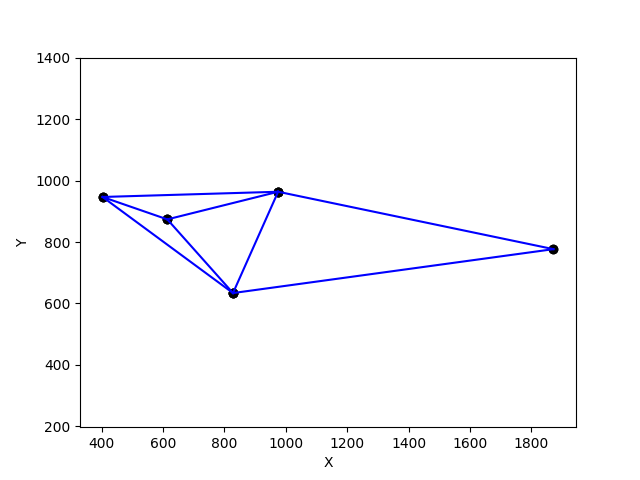
\includegraphics[width=0.41\textwidth]{alea4td.png}
	\caption{Contraseña gráfica de 5 puntos con una triángulación de Delaunay de 4 triángulos}
	\label{4TD}
\end{figure}

\subsection{Media muestral, desviación estándar y distribución del promedio de los ángulos máximos de los triángulos de Delaunay }
\textbf{Diseño del experimento \#2.1}

El procedimiento para el diseño de este experimento es similar al experimento \#1.1, con la principal diferencia de que, en este caso, las contraseñas gráficas aleatorias de 5 puntos, contenían 4 triángulos en su triangulación de Delaunay. Se trabajó con un total de 1000 contraseñas, y para cada una de ellas se calculó el promedio de los ángulos máximos en su respectiva triangulación de Delaunay. Finalmente, estos datos fueron recopilados en la base de datos DB.2.

%Para estimar la media muestral, desviación estándar  y distribución del promedio de los ángulos máximos de los triángulos de Delaunay en contraseñas gráficas de Passpoint, se generaron de manera aleatoria 1000 contraseñas gráficas formadas por 5 puntos ubicados en una imagen con resolución de 1920x1080. Para cada una de estas contraseñas, se construyó su correspondiente triangulación de Delaunay y se calculó el promedio de los ángulos máximos de los triángulos resultantes. Los 1000 promedios obtenidos fueron recopilados en una base de datos denominada BD.2.


\textbf{Resultados del experimento \#2.1}

Los datos analizados en BD.2 presentan una media de $116.74\degree$ y una desviación estándar de $13.411\degree$.
En la tabla \ref{teo_BD2}  se muestran las 6 distribuciones que más se ajustan a los datos encontrados en BD.2, encontrandose en el primer lugar Log-Logistic (3P) con los parámetros $\alpha=6.4824$, $\beta=46.461$ $\gamma=68.566$. Es importante destacar que la distribución Normal no se ajusta a los datos de BD.2, dado que se encuentra en la posición 31 de las distribuciones más ajustadas y, además rechaza los tres test de bondad de ajuste para todos los niveles de significación. En la figura \ref{4TD_BONDAD} se puede observar que los tres test de bondad de ajuste evaluados (Kolmogorov-Smirnov, Anderson-Darling y Chi-cuadrado) no rechazan la hipótesis nula de que los datos provienen de la distribución teórica Log-Logistic (3P) para ninguno de los niveles de significación analizados. Esto indica que los datos se ajustan adecuadamente a dicha distribución y un ejemplo de ello es la figura \ref{4TD_FDP}, que muestra la función de densidad de probabilidad de la misma. 
\begin{figure}[ht]
	\centering
	
	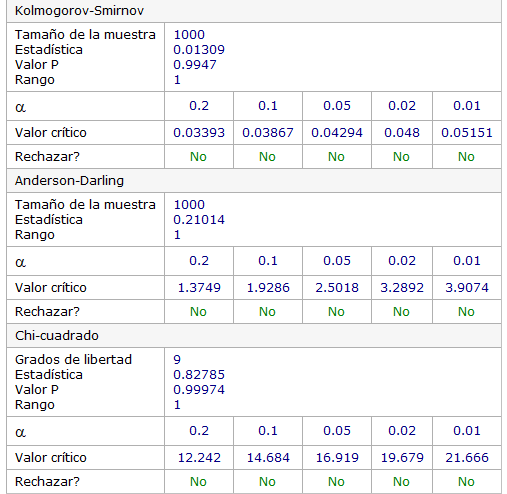
\includegraphics[width=0.5\textwidth]{4td_bondad.png}
	\caption{\textit{Test} de bondad de ajuste para la distribución Log-Logistic (3P) sobre BD.2.}
	\label{4TD_BONDAD}
\end{figure}




%Como se muestra en la figura \ref{4TD_BONDAD}, los tres test de bondad de ajuste evaluados (Kolmogorov-Smirnov, Anderson-Darling y Chi-cuadrado) no rechazan la hipótesis nula de que los datos provienen de la distribución teórica Log-Logistic (3P) para ninguno de los niveles de significación analizados. Esto indica que los datos se ajustan adecuadamente a dicha distribución.

Con base en este resultado, en el resto de la sección se asume que la muestra BD.2, y por extensión el promedio de los ángulos máximos de los triángulos de Delaunay, provienen de una distribución Log-Logistic (3P). Por lo tanto, se asume que las contraseñas que no cumplan con esta propiedad pueden considerarse como no aleatorias.
 
\begin{figure}[ht]
	\centering
	
	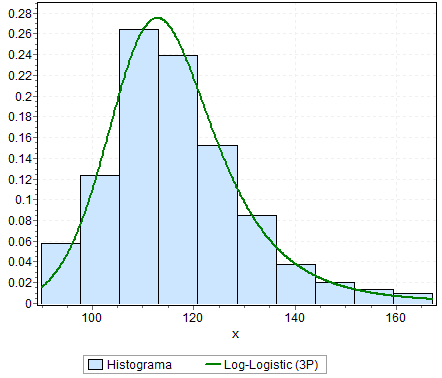
\includegraphics[width=0.6\textwidth]{4td_fdp.png}
	\caption{Función de densidad de probabilidad de la  distribución Log-Logistic (3P) para BD.2.}
	\label{4TD_FDP}
\end{figure}
\newpage

\subsection{\textit{Test} basado en el promedio de los ángulos máximos de triangulaciones de Delaunay con cuatro triángulos, para la detección de patrones DIAG y LINE en las contraseñas de PassPoint}

Dado que el promedio de los ángulos máximos de los triángulos de Delaunay sigue una distribución Log-Logistic, se propone un \textit{test} estadístico para identificar contraseñas con patrones DIAG y LINE. Este \textit{test} consiste en una prueba unilateral (cola derecha) basada en el promedio de los ángulos máximos de los triángulos de Delaunay.

Al igual que el \textit{test} previamente mencionado, este se fundamenta en la amplitud de los ángulos y no en la longitud de los lados ni en otras características que dependan del tamaño de la imagen. Por esta razón, este es válido para imágenes de cualquier tamaño siempre que mantengan una relación de aspecto de 16:9, ya que las dimensiones proporcionales garantizan que los triángulos correspondientes sean semejantes. La formalización del \textit{test} propuesto es la siguiente:
\begin{enumerate}
	\item Variable aleatoria X: promedio de los ángulos máximos de los triángulos de Delaunay en un conjunto de 5 puntos, con 4 triángulos en su triangulación.
	\item Estadígrafo: $X$
	
	\item Hipótesis nula: \[H_0:E(X)=0\]
	%\begin{itemize}
		%\item La contraseña gráfica seleccionada por el usuario es aleatoria si el promedio de los ángulos máximos de los triángulos de Delaunay es igual a 0
	%\end{itemize}
	
	
	\item Hipótesis alternativa: \[H_a:E(X)>0\]
	%\begin{itemize}
	%	\item 
	%\end{itemize}
	
	\item  Región de Rechazo: $\{z$:$Z>z_\alpha\}$,donde  $z_\alpha$ estará dado por la evaluación de los respectivos niveles de confianza \textit{p} en la  inversa de la función de distribución acumulada (FDA) de Log-Logistic (3P) con los parámetros obtenidos: 
	
	\[
	FDA(x; \alpha, \beta, \gamma) = \frac{1}{1 + \left( \frac{\beta}{x - \gamma} \right)^\alpha}, \quad x > \gamma
	\]
	\begin{itemize}
		\item  Para hallar la inversa de la función de distribución acumulada se debe despejar $x$:
		Para despejar \( x \), seguimos los pasos:
		
		Paso 1: Igualar \( F(x; \alpha, \beta, \gamma) \) a \( y \):
		\[
		y = \frac{1}{1 + \left( \frac{\beta}{x - \gamma} \right)^\alpha}
		\]
		
		Paso 2: Invertir la fracción:
		\[
		\frac{1}{y} = 1 + \left( \frac{\beta}{x - \gamma} \right)^\alpha
		\]
		
		Paso 3: Restar 1 de ambos lados:
		\[
		\frac{1}{y} - 1 = \left( \frac{\beta}{x - \gamma} \right)^\alpha
		\]
		
		Paso 4: Escribir con denominador común:
		\[
		\frac{1}{y} - 1 = \frac{1 - y}{y}
		\]
		Por lo tanto:
		\[
		\frac{1 - y}{y} = \left( \frac{\beta}{x - \gamma} \right)^\alpha
		\]
		
		Paso 5: Elevar ambos lados a la \( \frac{1}{\alpha} \) potencia:
		\[
		\left( \frac{1 - y}{y} \right)^{\frac{1}{\alpha}} = \frac{\beta}{x - \gamma}
		\]
		
		Paso 6: Invertir la fracción de la derecha:
		\[
		x - \gamma = \frac{\beta}{\left( \frac{1 - y}{y} \right)^{\frac{1}{\alpha}}}
		\]
				
		Paso 7: Pasar \( \left( \frac{1 - y}{y} \right)^{\frac{1}{\alpha}} \) multiplicando a \( \beta \):
		\[
		x - \gamma = \beta \cdot \left( \frac{1 - y}{y} \right)^{-\frac{1}{\alpha}}
		\]
		
		Paso 8: Simplificar \( x \):
		\[
		x = \gamma + \beta \cdot \left( \frac{1 - y}{y} \right)^{-\frac{1}{\alpha}}
		\]
		
		\[
		x = \gamma + \beta \cdot \left( \frac{1}{\frac{1}{y}-1} \right)^{\frac{1}{\alpha}}
		\]
		
		Finalmente, sustituyendo \( y = p \), la solución general es:
		\[
		 z_\alpha = \gamma + \beta \cdot \left( \frac{1}{\frac{1}{p}-1} \right)^{\frac{1}{\alpha}}
		\]
		
		
	\end{itemize}
	\item Criterio de decisión
	\begin{itemize}
		\item Para los cinco niveles de significación establecidos, se decide que la contraseña gráfica seleccionada por el usuario no sigue un patrón aleatorio si su promedio de los ángulos máximos de los triángulos de Delaunay  pertenece a la región crítica. 
	\end{itemize}
\end{enumerate}
\subsection{Implementación del \textit{Test} propuesto }

Al igual que  la implementación del \textit{test} encontrado en la sección 2.1.3, para este, se toman las coordenadas \((x_i, y_i)\) de cada uno de los \(p_i\) puntos, \(i = 1, \ldots, 5\) como valores de entrada. A partir de estos puntos, se construye la triangulación Delaunay utilizando la función \textit{Delaunay} de scipy.spatial.
Luego, la longitud de los lados de cada triángulo se determina por la distancia euclidiana de dos a dos de los puntos que lo forman y para encontrar el valor de los ángulos de cada triángulo, se aplica la Ley de los Cosenos. Una ves obtenidos todos los ángulos, se busca el promedio de los ángulos máximos  de la triangulación de Delaunay correspondiente.  Este va a set el valor de el estadígrafo \(X\), donde la hipótesis nula se rechaza dependiendo de si  \(X\) pertenece a la región de rechazo para el \(\alpha\) establecido. 

Una posible implementación de esta prueba en python sería:



%Es necesario encontrar el máximo de estos tres ángulos \(\theta\), \(\phi\), y \(\psi\). Es análogo para los triángulos restantes de la triangulación Delaunay. Una vez que se hayan obtenido los ángulos máximos de la triangulación Delaunay, se calcula su promedio, con el cual se obtiene el valor de la estadígrafo \(X\). La hipótesis nula se rechaza dependiendo de si la estadística \(X\) pertenece a la región de rechazo para el \(\alpha\) establecido. Una posible implementación de esta prueba en python sería:

\begin{itemize}
	\item points 5 puntos de la contraseña.
	\item alpha, beta, gamma: parámetros de la distribución Log-Logistic (3P) obtenida.
	\item nivel\_sig: nivel de significación escogido.
	
\end{itemize}
La implementación retorna 0 si se rechaza la hipótesis nula y 1 en caso contrario. 





\begin{lstlisting}
def test(points, alpha, beta, gamma,nivel_sig):
	triangulation=Delaunay(points)
	angles=[]
	for i in triangulation:
		a=distancia_puntos(points[i[0]],points[i[1]])
		b=distancia_puntos(points[i[1]],points[i[2]])
		b=distancia_puntos(points[i[2]],points[i[0]])
		angles.append(angle_max(a,b,c))     
	X=mean(angles) 
	rg= beta * ((1 / (1 / (1-nivel_sig) - 1)) ** (1 / alpha)) + gamma
	if X>rg:
		return 0
	else:
		return 1

def distancia_puntos(punto1, punto2):
	return math.sqrt((punto1[0] - punto2[0])**2 +
	 (punto1[1] - punto2[1])**2)

def angle_max(distancia_ab, distancia_bc, distancia_ca):
	angulo_A = math.degrees(math.acos(
	(distancia_bc**2 + distancia_ca**2 - distancia_ab**2) 
	/ (2 * distancia_bc * distancia_ca)
	))
	angulo_B = math.degrees(math.acos(
	(distancia_ca**2 + distancia_ab**2 - distancia_bc**2) 
	/ (2 * distancia_ca * distancia_ab)
	))
	angulo_C = 180 - angulo_A - angulo_B  
	return max(angulo_A, angulo_B, angulo_C)
\end{lstlisting}

En cuanto a la complejidad, las funciones \textit{distancia\_puntos} y \textit{angle\_max} solo poseen operaciones elementales por lo que su complejidad es \textit{O(1)}. La función test en su primera línea hace un llamado a la función  \textit{Delaunay} (línea 2) de \textit{scipy.spatial}, esta posee una complejidad de \textit{O(N logN)} debido a que el algoritmo subyacente utilizado por \textit{Scipy} es el algoritmo de \textit{Qhull}. Seguido en el algoritmo se itera por la triangulación obtenida (líneas 4-8), la cual poseen como máximo \textit{n} triángulos , dentro de cada iteración se hacen llamados a las  funciones \textit{distancia\_puntos} y \textit{angle\_max}  que son \textit{O(1)}, por tanto el costo del iterador es \textit{O(N)}. Las operaciones restantes son \textit{O(1)} (líneas 9-14) ,por tanto el costo total sería \textit{O(1)}+\textit{O(N)}+\textit{O(N logN)}=\textit{O(N logN)} por ley de la suma.

\subsection{Validación del \textit{test} propuesto}

%Con el objetivo de validar la eficacia del \textit{test} se realizó una estimación de la probabilidad de cometer errores de tipo I (falsos positivos) y de tipo II (falsos negativos).
Para evaluar la precisión y confiabilidad del test, se llevó a cabo una estimación de la probabilidad de cometer errores en la clasificación. Por lo que se estimó la probabilidad de que el test cometa  errores de tipo I (falsos positivos) y de tipo II (falsos negativos)

\textbf{Diseño del experimento \#2.2 : Estimación de la probabilidad de cometer un error de tipo I} 

Para estimar la probabilidad de que la prueba decida que la contraseña gráfica contiene un patrón DIAG o LINE cuando, en verdad, sigue un patrón aleatorio (error de tipo I o falsos positivos), se generó una base de datos llamada BD.2.RANDOM con 10 000 contraseñas gráficas aleatorias sobre la imagen. El \textit{test} descrito en la sección 2.2.3, se aplicó a cada una de estas contraseñas gráficas, obteniendo como límites inferiores de la región crítica a  $rg \in \{$126.105, 133.772, 141.739, 153.254, 162.959$\}$ para los respectivos  niveles de significación $\alpha \in \{0.2, 0.1 0.05, 0.02 , 0.01\}$ .

\begin{table}[h!]
	\centering
	\begin{tabular}{|c|ccccc|}
		\hline
		$\alpha$ &  0.2 & 0.1 & 0.05 & 0.02 &  0.01 \\
		\hline
		$\hat{\alpha}$ & 0.2032 & 0.1083 & 0.0552 & 0.0134 & 0.0034 \\
		\hline
	\end{tabular}
	\caption{Estimación de la probabilidad ($\hat{\alpha}$) del error de tipo I derivado de la prueba.}
	\label{tab:error1-prob1}
\end{table}

\textbf{Resultados del experimento \#2.2}

Las probabilidades estimadas de cometer un error de tipo I ($\hat{\alpha}$) mediante el \textit{test} poseen gran similitud  a las probabilidades teóricas preestablecidas ($\alpha$),véase en la figura \ref{Teorico vs Observado}.
\begin{figure}[ht]
	\centering
	
	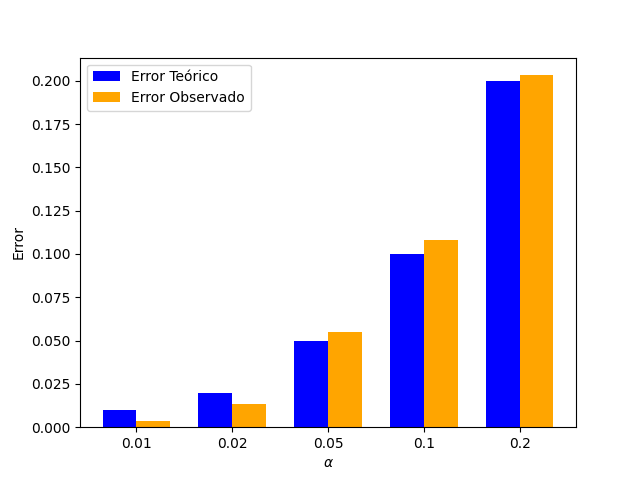
\includegraphics[width=0.8\textwidth]{4td_teo_obs.png}
	\caption{Comparación entre las probabilidades teóricas ($\alpha$) y estimadas ($\hat{\alpha}$) de cometer un error de tipo I }
	\label{Teorico vs Observado1}
\end{figure}\\

\textbf{Experimento \#2.3: Estimación de la probabilidad de cometer un error de tipo II}

Para estimar la probabilidad $\hat{\beta}$ de que el \textit{test} detecte una contraseña gráfica como aleatoria cuando sigue un patrón DIAG o LINE (error tipo II o falsos negativos), se crearon 3 bases de datos que en conjunto contienen 30 000 contraseñas gráficas de 5 puntos que siguen patrones DIAG y LINE :
\begin{itemize}
	\item BD.DIAG\_LINE.2.3.1: 10 000 contraseñas gráficas que siguen patrones DIAG o LINE con una anchura máxima entre dos segmentos consecutivos de 15\degree. Base de datos con mayor nivel de suavidad. 
	\item BD.DIAG\_LINE.2.3.2: 10 000 contraseñas gráficas que siguen patrones DIAG o LINE con una anchura máxima entre dos segmentos consecutivos que varia entre 15\degree y 30\degree. Base de datos medianamente suave. 
	\item BD.DIAG\_LINE.2.3.3: 10 000 contraseñas gráficas que siguen patrones DIAG o LINE con una anchura máxima entre dos segmentos consecutivos que varia entre 30\degree y 45\degree. Base de datos con menor nivel de suavidad.
\end{itemize}
\textbf{Resultados del experimento \#2.3}

Los resultados obtenidos por el \textit{test}  para cada una de las bases de datos y los  niveles de significación preestablecidos se muestran en la tabla \ref{tab:error2-prob1}.

\begin{table}[h!]
	\centering
	\begin{tabular}{|c|ccc|}
		\hline
		$\alpha$& BD.DIAG\_LINE.2.3.1 & BD.DIAG\_LINE.2.3.2 & BD.DIAG\_LINE.2.3.3  \\
		\hline
		0.2 & 0     & 0          & 0.0001     \\
		0.1 & 0     & 0          & 0.0174     \\
		0.05 & 0     & 0   		& 0.2577     \\
		0.02 & 0     & 0.0642    & 0.9798     \\
		0.01 & 0     & 0.8688    & 1.0000     \\
		\hline
	\end{tabular}
	\caption{Estimación de la probabilidad ($\hat{\beta}$) del error de tipo II derivado de la prueba.}
	\label{tab:error2-prob1}
\end{table}
El test propuesto durante este experimento mostró una alta capacidad para detectar las contraseñas encontradas en BD.DIAG\_LINE.2.3.1, pues detectó el 100\% de estas para todos los niveles de significación, en BD.DIAG\_LINE.2.3.2 detectó el 100\% para los niveles de significación $\alpha \in \{0.2, 0.1, 0.05\}$ y 93\% para $\alpha=0.02$ . Para las contraseñas de BD.DIAG\_LINE.2.3.3 no se obtuvieron buenos resultados, dado que para los casos de $\alpha \in \{ 0.05, 0.02, 0.01\}$ solo detectó el 74\%, 2\% y 0\% respectivamente. 

\section{Contraseñas con 5 triángulos en su triangulación de Delaunay }
Como mismo se definió en las secciones anteriores, en esta  cuando hacemos referencia a el promedio de los ángulos máximos de los triángulos de Delaunay  de las contraseñas gráficas en PassPoint, nos referiremos a las contraseñas que posean 5 triángulos en su triangulación de Delaunay\ref{5TD}. 

\begin{figure}[ht]
	\centering
	
	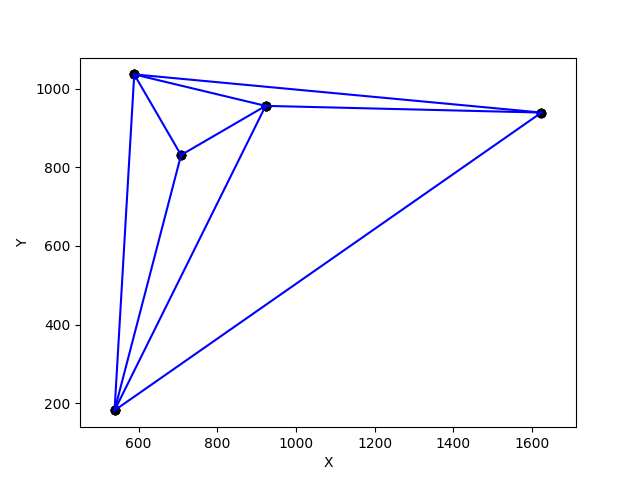
\includegraphics[width=0.41\textwidth]{alea5td.png}
	\caption{Contraseña gráfica de 5 puntos con una triangulación de Delaunay de 5 triángulos.}
	\label{5TD}
\end{figure}

\subsection{Media muestral, desviación estándar y distribución del promedio de los ángulos máximos de los triángulos de Delaunay  ç}
\textbf{ Diseño del experimento \#3.1}

De manera similar a al diseño de los experimentos \#1.1 y \#2.1, en este experimento se generaron de manera aleatoria 1000 contraseñas gráficas de 5 puntos en una imagen de 1920x1080, pero con la condición de que cada una de ellas contenga 5 triángulos en su triangulación de Delaunay. A cada contraseña se le construyó su respectiva triangulación y se halló el promedio de los ángulos máximos de los triángulos de la misma. A la base de datos que contiene los 1000 promedios se le denominó BD.3

%De igual manera que en las secciones anteriores para estimar la distribución del promedio de los ángulos máximos de los triángulos de Delaunay para contraseñas gráficas en PassPoint, se generaron de manera aleatoria 1000 contraseñas gráficas de 5 puntos en una imagen de 1920x1080. Para cada una de estas contraseñas se  construyó  su correspondiente triangulación  de Delaunay  y se  determinó el promedio  de los ángulos máximos de su triangulación de Delaunay resultante. La base de datos que contiene los 1000 promedios se le denominó BD.3.


\textbf{Resultados del experimento \#3.1}

Los resultados obtenidos presentan una media de 132.65\degree y una desviación estándar de 9.43\degree. En la tabla \ref{teo_BD3}  se muestran las 6 distribuciones que más se ajustan a los datos encontrados en BD1.1, encontrándose en el primer lugar Log-Logistic (3P) con los parámetros $\alpha=5.8577$, $\beta=28.592$ $\gamma=102.72$. Al igual que en los resultados de los experimentos \#1.1 y \#2.1, la distribución Normal no se encontró entre las más ajustadas, al contrario de como se esperaba, ocupando el lugar 34 y rechazando los tres test de bondad de ajuste para todos los niveles de significación. En la figura \ref{5TD_BONDAD} se  muestran los datos de tres de los \textit{test} de bondad de ajuste (Kolmogorov-Smirnov, Anderson-Darling y Chi-cuadrado) aplicados a la distribución obtenida sobre los datos contenidos en BD.3, donde no se rechaza la hipótesis nula de que los datos provienen de la distribución teórica Log-Logistic (3P) en ningún nivel de significación evaluado, indicando un buen ajuste hacia la misma. Un ejemplo de este ajuste es la figura \ref{5TD_FDP}, que muestra la función de densidad de probabilidad de la misma. 
\begin{figure}[ht]
	\centering
	
	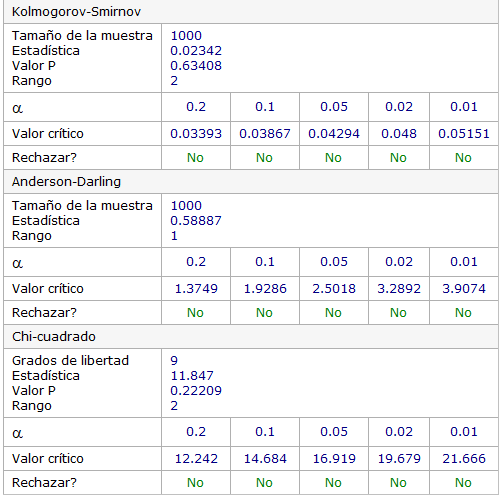
\includegraphics[width=0.5\textwidth]{5td_bondad.png}
	\caption{\textit{Test} de bondad de ajuste para la distribución Log-Logistic (3P) sobre BD.3}
	\label{5TD_BONDAD}
\end{figure}
         
%Como se observa en la figura  \ref{5TD_BONDAD}, para los tres métodos de bondad de ajuste (Kolmogorov-Smirnov, Anderson-Darling y Chi-cuadrado), no se rechaza la hipótesis nula de que los datos provienen de la distribución teórica Log-Logistic (3P) en ningún nivel de significación evaluado, indicando un buen ajuste hacia la misma.

A partir de este resultado, en el resto de la sección se asume que la muestra  BD.3 y, por tanto, el promedio de los ángulos máximos de los triángulos de Delaunay en contraseñas con 5 triángulos en su triangulación  proceden de una distribución Log-Logistic (3P), por tanto se puede asumir que que las contraseñas que incumplan esta propiedad no son aleatorias.
\begin{figure}[ht]
	\centering
	
	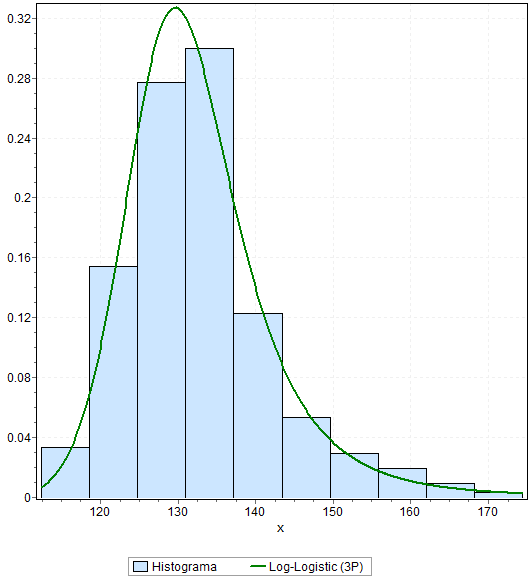
\includegraphics[width=0.5\textwidth]{5td_fdp.png}
	\caption{Función de densidad de probabilidad de la  distribución Log-Logistic (3P) para BD.3}
	\label{5TD_FDP}
\end{figure}

\newpage
\subsection{\textit{Test} basado en el promedio de los ángulos máximos de triangulaciones de Delaunay con cinco triángulos, para la detección de patrones DIAG y LINE en las contraseñas de PassPoint}
Como la distribución   obtenida en el experimento \#3.1 es la misma que la obtenida en la sección 2.2.1, tanto el \textit{test} propuesto como su implementación  serían el mismo, solo que con otros parámetros.

%Dado  que el el promedio de los ángulos máximos de los triágulos de Delanunay distribuye Log-Logistic, se propone un  test estadístico para seleccionar contraseñas con patrones DIAG y LINE. La propuesta consiste en un test de una cola( Derecha) basado en el promedio de los ángulos máximos de los triángulos de Delanunay .
%Al igual que  el test anterior, este se basa en la anchura de los ángulos y no en la longitud en sí de los lados u otra característica que varie con el tamaño de la imagen, por lo que será válida para todos los tamaños de imágenes con una relación de 16:9. Dado que las imágenes con esta relación tendrán dimensiones proporcionales iguales y sus triángulos correspondientes serán proporcionales: la prueba propuesta puede formalizarse como sigue:

\begin{enumerate}
	\item Variable aleatoria X: promedio de los ángulos máximos de los triángulos de Delaunay en un conjunto de 5 puntos, con 5 triángulos en su triangulación.
	\item Estadígrafo: $X$
	
	\item Hipótesis nula: \[H_0:E(X)=0\]
	%\begin{itemize}
	%\item La contraseña gráfica seleccionada por el usuario es aleatoria si el promedio de los ángulos máximos de los triángulos de Delaunay es igual a 0
	%\end{itemize}
	
	
	\item Hipótesis alternativa: \[H_a:E(X)>0\]
	%\begin{itemize}
	%	\item 
	%\end{itemize}
	
	\item  Región de Rechazo: $\{z$:$Z>z_\alpha\}$,donde $\alpha$ es el nivel de significación establecido por el usuario,  $z_\alpha$  el valor que estará dado por la evaluación de los respectivos niveles de confianza \textit{p} en la  inversa de la función de distribución acumulada (FDA) de Log-Logistic (3P) con los parámetros obtenidos: 
	
	\[
	FDA(x; \alpha, \beta, \gamma) = \frac{1}{1 + \left( \frac{\beta}{x - \gamma} \right)^\alpha}, \quad x > \gamma
	\]
	\begin{itemize}
		\item inversa de FDA evaluada en p como se demostró en la subsección 2.2.2.
		
	
		\[
		rg = \gamma + \beta \cdot \left( \frac{1}{\frac{1}{p}-1} \right)^{\frac{1}{\alpha}}
		\]
		
	\end{itemize}
	\item Criterio de decisión:
	\begin{itemize}
		\item Para los cinco niveles de significación establecidos, se decide que la contraseña gráfica seleccionada por el usuario no sigue un patrón aleatorio si su promedio de los ángulos máximos de los triángulos de Delaunay  pertenece a la región crítica. 
	\end{itemize}
\end{enumerate}
\subsection{Implementación del \textit{test} propuesto :}
En cuanto  la implementación del \textit{test} , como se explicó en la sección 2.3.2 es el mismo que se utilizó en la sección 2.2.3, solo que cambiando los parámetros por los obtenidos en la sección 2.3.1, por lo tanto su nivel de complejidad es el mismo, \textit{O(N logN)}.

\begin{lstlisting}
	def test(points, alpha, beta, gamma,nivel_sig):
	triangulation=Delaunay(points)
	angles=[]
	for i in triangulation:
	a=distancia_puntos(points[i[0]],points[i[1]])
	b=distancia_puntos(points[i[1]],points[i[2]])
	b=distancia_puntos(points[i[2]],points[i[0]])
	angles.append(angle_max(a,b,c))     
	X=mean(angles) 
	rg= beta * ((1 / (1 / (1-nivel_sig) - 1)) ** (1 / alpha)) + gamma
	if X>rg:
	return 0
	else:
	return 1
	
	def distancia_puntos(punto1, punto2):
	return math.sqrt((punto1[0] - punto2[0])**2 +
	(punto1[1] - punto2[1])**2)
	
	def angle_max(distancia_ab, distancia_bc, distancia_ca):
	angulo_A = math.degrees(math.acos(
	(distancia_bc**2 + distancia_ca**2 - distancia_ab**2) 
	/ (2 * distancia_bc * distancia_ca)
	))
	angulo_B = math.degrees(math.acos(
	(distancia_ca**2 + distancia_ab**2 - distancia_bc**2) 
	/ (2 * distancia_ca * distancia_ab)
	))
	angulo_C = 180 - angulo_A - angulo_B  
	return max(angulo_A, angulo_B, angulo_C)
\end{lstlisting}

\subsection{Validación del \textit{test} propuesto}
Al igual que en secciones anteriores para validar la efectividad de este test se realizó una estimación de la probabilidad de que este cometa errores de tipo I y tipo II
	 
\textbf{Diseño del experimento \#3.2 : Estimación de la probabilidad de cometer un e error de tipo I} 

Para estimar la probabilidad de que el \textit{test} decida que la contraseña gráfica contiene un patrón DIAG o LINE cuando,en verdad, sigue un patrón aleatorio (error de tipo I o falsos positivos), se generó una base de datos llamada BD.3.RANDOM con 10 000 contraseñas gráficas aleatorias sobre la imagen. El \textit{test} descrito en la sección 2.2.3, se le aplicó a cada una de estas contraseñas gráficas, obteniendo como límites inferiores de la región crítica a $rg \in \{$138.946, 144.325, 149.985, 158.283, 165.372$\}$  para los respectivos  niveles de significación $\alpha \in \{$0.2, 0.1 0.05, 0.02 , 0.01$\}$.



\textbf{Resultados del experimento \#3.2}

Las probabilidades estimadas de cometer un error de tipo I ($\hat{\alpha}$) mediante el \textit{test} poseen gran similitud  a las probabilidades teóricas preestablecidas ($\alpha$),véase en la figura \ref{Teorico vs Observado3}.
\begin{table}[h!]
	\centering
	\begin{tabular}{|c|ccccc|}
		\hline
		$\alpha$ & 0.2 &   0.1 &  0.05 &  0.02 &  0.01 \\
		\hline
		$\hat{\alpha}$ & 0.1943 & 0.1074 & 0.057 & 0.0181 & 0.0051 \\
		\hline
	\end{tabular}
	\caption{Estimación de la probabilidad ($\hat{\alpha}$) del error de tipo I derivado de la prueba.}
	\label{tab3:error1-prob1}
\end{table}
\begin{figure}[ht]
	\centering
	
	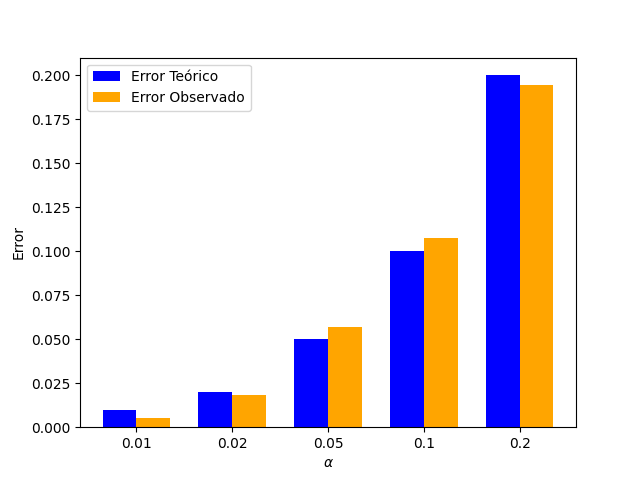
\includegraphics[width=0.8\textwidth]{5td_teo_obs.png}
	\caption{Comparación entre las probabilidades teóricas ($\alpha$) y estimadas ($\hat{\alpha}$) de cometer un error de tipo I. }
	\label{Teorico vs Observado3}
\end{figure}\\
\newpage
\textbf{Diseño del experimento \#3.2: Estimación de la probabilidad de cometer un e error de tipo II}

Para estimar la probabilidad $\hat{\beta}$ de que el \textit{test} detecte una contraseña gráfica como aleatoria cuando sigue un patrón DIAG o LINE (error tipo II o falsos negativos), se crearon 3 bases de datos que en conjunto contienen 30 000 contraseñas gráficas de 5 puntos que siguen patrones DIAG y LINE :
\begin{itemize}
	\item BD.DIAG\_LINE.3.3.1: 10 000 contraseñas gráficas que siguen patrones DIAG o LINE con una anchura máxima entre dos segmentos consecutivos de 15\degree. Base de datos con mayor nivel de suavidad. 
	\item BD.DIAG\_LINE.3.3.2: 10 000 contraseñas gráficas que siguen patrones DIAG o LINE con una anchura máxima entre dos segmentos consecutivos que varia entre 15\degree y 30\degree. Base de datos medianamente suave.
	\item BD.DIAG\_LINE.3.3.3: 10 000 contraseñas gráficas que siguen patrones DIAG o LINE con una anchura máxima entre dos segmentos consecutivos que varia entre 30\degree y 45\degree. Base de datos con menor nivel de suavidad.
\end{itemize}
\textbf{Resultados del experimento \#3.3}

Los resultados obtenidos por el \textit{test}  para cada una de las bases de datos y los  niveles de significación preestablecidos, se muestran en las tablas \ref{tab3:error2-prob1}.

\begin{table}[h!]
	\centering
	\begin{tabular}{|c|ccc|}
		\hline
		$\alpha$& BD.DIAG\_LINE.3.3.1 & BD.DIAG\_LINE.3.3.2 & BD.DIAG\_LINE.3.3.3  \\
		\hline
		0.2 & 0     & 0          & 0     \\
		0.1 & 0     & 0          & 0.0094     \\
		0.05 & 0     & 0   		& 0.1439     \\
		0.02 & 0     & 0.0019   & 0.9753     \\
		0.01 & 0     & 0.7365    & 1.0000     \\
		\hline
	\end{tabular}
	\caption{Estimación de la probabilidad ($\hat{\beta}$) del error de tipo II derivado de la prueba.}
	\label{tab3:error2-prob1}
\end{table}
El \textit{test} propuesto durante este experimento mostró una alta capacidad para detectar las contraseñas encontradas en BD.DIAG\_LINE.3.3.1, pues detectó el 100\% de estas para todos los niveles de significación, en BD.DIAG\_LINE.3.3.2 detectó el 100\% para los niveles de significación $\alpha \in \{$0.2, 0.1, 0.05$\}$ y 99\% para $\alpha=0.02$ . Para las contraseñas de BD.DIAG\_LINE.2.3.3 los resultados fueron mejores que en los dos \textit{test} anteriores pues para los niveles de significación $\alpha \in \{$0.2, 0.1 0.05$\}$ la prueba detectó el 100\%, 99\% y 85\% en cada caso.



\section{Discusión de los resultados de los \textit{test} anteriores}
Los experimentos \#1.1, \#2.1 y \#3.1 muestran que a medida que aumenta la cantidad de triángulos en las triangulaciones de Delaunay, aumenta la media de los promedios de los ángulos máximos de las triangulaciones de Delaunay y disminuye la desviación estándar de los mismos. En el caso de los experimentos encontrados en las secciones 2.1.4, 2.2.4 y 2.3.4, muestran la eficacia de los \textit{test} propuestos  para detectar contraseñas que sigan patrones DIAG o LINE. Los patrones cuyos ángulos están comprendidos entre 0\degree y 15\degree, que son los que más se aproximan a la forma típica de los patrones DIAG y LINE que han sido simulados en las bases de datos BD.DIAG\_LINE.1.3.1, BD.DIAG\_LINE.2.3.1 y BD.DIAG\_LINE.3.3.1 son detectados por el \textit{test} propuesto con una efectividad del 100\% para todos los niveles de significación. Mientras que para las contraseñas con ángulos comprendidos entre 15\degree y 30\degree se logró detectar el 100\% para los niveles de significación $\alpha \in \{$0.2, 0.1, 0.05$\}$, excepto en BD.DIAG\_LINE.1.3.2, que para $\alpha$=0.05 logró un 99.7\%. En el caso de $\alpha$=0.02 se logró detectar el 90\%, 93\% y 99\% para BD.DIAG\_LINE.1.3.2, BD.DIAG\_LINE.2.3.2 y BD.DIAG\_LINE.3.3.2 respectivamente. Donde más se evidencia la diferencia entre  el primer \textit{test} y los dos últimos es en las contraseñas detectadas cuando la amplitud entre segmentos se encuentra entre 30\degree a 45\degree, los resultados se muestran en la tabla \ref{tab:error2-30-45}. Los resultados más significante son los obtenidos para los niveles de significación $\alpha \in \{$0.2, 0.1$\}$, pues en   BD.DIAG\_LINE.2.3.3 y BD.DIAG\_LINE.3.3.3  se logra detectar prácticamente el 100\% de las contraseñas para $\alpha$=0.2, y para$\alpha$=0.1 se logró detectar 98\% y 99\%, notable diferencia con el 73\% que se detecta el \textit{test} 1 en BD.DIAG\_LINE.1.3.3. En el caso de los restantes niveles de significación no se obtuvieron los resultados esperados.
\begin{table}[h!]
	\centering
	\begin{tabular}{|c|ccc|}
		\hline
		$\alpha$& BD.DIAG\_LINE.1.3 & BD.DIAG\_LINE.2.3 & BD.DIAG\_LINE.3.3  \\
		\hline
		0.2 & 0.0571     & 0.0001     & 0     \\
		0.1 & 0.2721      & 0.0174    & 0.0094     \\
		0.05& 0.5222    & 0.2577  & 0.1439     \\
		0.02& 0.8508     & 0.9798    & 0.9753     \\
		0.01& 0.9871     & 1.0000     & 1.0000     \\
		\hline
	\end{tabular}
	\caption{Estimación de la probabilidad ($\hat{\beta}$) de error tipo II para contraseñas con ángulos entre segmentos de $30\degree$ a $45\degree$.}
	\label{tab:error2-30-45}
\end{table}

En cuanto a los falsos positivos  el segundo \textit{test} tuvo ligeramente mayor eficacia que el tercer \textit{test} mostrando gran similitud entre ambos, mientras que el primer \textit{test} las probabilidades estimadas son ligeramente superiores que las preestablecidas, véase en la tabla \ref{tab:error1}
\begin{table}[h!]
	\centering
	\begin{tabular}{|c|ccc|}
		\hline
		$\alpha$& \textit{test} 1 & \textit{test} 2 & \textit{test} 3  \\
		\hline
		0.2 &  0.2221    & 0.2032    &  0.1943   \\
		0.1 &  0.1178    & 0.1083    &  0.1074   \\
		0.05&  0.0605    & 0.0552    &  0.057   \\
		0.02&  0.0251    & 0.0134    &  0.0181   \\
		0.01&  0.0132    & 0.0034    &  0.0051   \\
		\hline
	\end{tabular}
	\caption{Estimación de la probabilidad ($\hat{\alpha}$) de error tipo I para cada \textit{test}.}
	\label{tab:error1}
\end{table}
\section{Comparación del los test propuestos con el encontrado en  \cite{13}}
Un resumen de los resultados del \textit{test} propuesto en \cite{13} se encuentran en la sección 1.4.2. Como era de esperarse la media del test propuesto en \cite{13}, esta contenida en los intervalos de las medias de los test realizados, específicamente entre la media de los experimentos \#1.1 y \#2.1, correspondientes a 3 y 4 triángulos respectivamente, demostrando que las contraseñas con 5 triangulaciones son las más escasas. En la tabla \ref{tab:erro1-sensor} se encuentra la estimación de la probabilidad de cometer un error de tipo I por el \textit{test} propuesto en \cite{13}, realizando una comparación entre esta tabla y la tabla \ref{tab:error1} se observa que la probabilidad de los \textit{test} 2 y 3 de cometer esto error es menor, mientras que con respecto al \textit{test} 1 posee más similitud. 
\begin{table}[h!]
	\centering
	\begin{tabular}{|c|ccccc|}
		\hline
		$\alpha$ & $\alpha = 0.2$ & $\alpha = 0.1$ & $\alpha = 0.05$ & $\alpha = 0.02$ & $\alpha = 0.01$ \\
		\hline
		$\hat{\alpha}$ & 0.2146 & 0.1098 & 0.0558 & 0.0253 & 0.0147 \\
		\hline
	\end{tabular}
	\caption{Estimación de la probabilidad ($\hat{\alpha}$) del error de tipo I del \textit{test} propuesto en \cite{13}.}
	\label{tab:erro1-sensor}
\end{table}

En cuanto a los falsos negativos, el \textit{test} propuesto en \cite{13} es superior a los \textit{test} realizados en este trabajo, pues para contraseñas con ángulos entre segmentos de  $0\degree$ a $30\degree$ detectó el 100\% de las contraseñas para todos los niveles de significación mientras que en los \textit{test} realizados para los niveles de significación  $\alpha \in \{$0.02, 0.01$\}$ ya no se cumplía. Para el caso de las contraseñas que poseen ángulos entre segmentos de $30\degree$ a $45\degree$ el \textit{test} propuesto en \cite{13} para los niveles de significación $\alpha \in \{$0.2, 0.1$\}$ detectó 100\% y para $\alpha \in \{$0.5, 0.02, 0.01$\}$ la eficacia fue aproximadamente  del 88\%, 42\% y 16\% respectivamente, comparando estos resultados con los que se encuentran en la tabla \ref{tab:error2-30-45} se muestra una mayor eficacia para todos los niveles de significación por parte del \textit{test} propuesto en \cite{13}.

Debido a los buenos resultados del test propuesto en \cite{13}, sobre todo para contraseñas que sus ángulos entre segmentos se encuentran entre $0\degree$ y $30\degree$, se puede decir que este y los test propuestos en este trabajo son redundantes, es decir, las contraseñas detectadas por los test propuestos también serían detectadas por el encontrado en \cite{13}. Una aplicación conjunta no aumentaría significativamente la efectividad, sino que sería menos eficiente computacionalmente.

%Se asume que los test propuestos y el encontrado en \cite{13} son redundantes, es decir, que las contraseñas detectadas por los test de este trabajo también son detectadas por el test propuesto en \cite{13}, esto lo demuestran los buenos resultados resultados de este último. Una aplicación conjunta de los mismos no aumentaría significativamente la efectividad, sino disminuiría la eficacia    
\chapter*{Conclusiones y Recomendaciones }
\addcontentsline{toc}{chapter}{Conclusiones y Recomendaciones}
En este trabajo se analizó cómo distribuyen los promedios de los ángulos máximos de los triángulos de las triangulaciones de Delaunay para distintos números de triángulos en su triangulación en contraseñas de 5 puntos. Para ello, se crearon tres bases de datos (BD.1, BD.2 y BD.3), cada una con 1000 contraseñas aleatorias de 5 puntos en una imagen de 1920x1080. A partir de estas configuraciones, se construyeron sus respectivas triangulaciones de Delaunay y se calcularon los promedios de los ángulos máximos de los triángulos en cada caso. Usando el software EasyFit, se estimaron las distribuciones de estos valores, encontrando que para BD.1, correspondiente a contraseñas con 3 triángulos, la distribución que mejor se ajusta es la \textit{Johnson SB}, mientras que para BD.2, con contraseñas de 4 triángulos, y BD.3, con contraseñas de 5 triángulos, la distribución más adecuada en ambos casos es la Log-Logistic (3P). Se obtuvo que para ningún número de  triángulos en la triangulación, el promedio de los ángulos máximos de los triángulos de Delaunay  se ajustan a una distribución Normal, rechazando los tres \textit{test} de bondad de ajuste para todos los niveles de significación en cada caso, resultando lo contrario a lo que se esperaba. Sin embargo, a partir de las distribuciones a las que fueron ajustadas los datos, en cada caso, fue posible construir test estadístico para detectar patrones DIAG y LINE en las contraseñas gráficas del escenario PassPoint y se desarrolló su implementación en Python. Tanto el \textit{test} como su implementación son aplicables a imágenes de cualquier tamaño que mantengan una relación de aspecto 16:9, ya que estas dimensiones proporcionales aseguran que los triángulos generados sean semejantes. 

Para estimar los falsos positivos, se crearon tres bases de datos aleatorias de prueba, cada una con 10 000 contraseñas, clasificadas según el número de triángulos en sus triangulaciones de Delaunay. Los errores tipo I cometidos estimados en cada caso estuvieron muy cerca de los valores teóricos preestablecidos, e incluso fueron menores para la mayoría de los niveles de significación evaluados. En cuanto a los falsos negativos o errores tipo II, para cada \textit{test} se construyeron 30 000 contraseñas con sus respectivas cantidades de triángulos en  su triangulación, divididas según la amplitud de los segmentos consecutivos de las mismas. Para las contraseñas donde  la amplitud de sus segmentos consecutivos estaba entre $0\degree$ y $15\degree$, se logró detectar el 100\%, en el caso de las que oscilaban entre $15\degree$ y $30\degree$  se logró detectar el 100\% para los niveles de significación $\alpha \in \{$0.02, 0.01$\}$. En el caso de las contraseñas con ángulos entre segmentos de $30\degree$ a $45\degree$  los resultados no fueron los esperados, pues a nivel general, para los tres \textit{test}   la eficacia es muy baja.

En la comparación con el \textit{test} propuesto en \cite{13}, se demostró la superioridad de este  a los realizados en este trabajo, a pesar de trabajar el promedio de los ángulos máximos de los triángulos de Delaunay de manera general, es decir, sin tener en cuenta la cantidad de triángulos en  la triangulación. Este detecta el 100\% de las contraseñas que poseen los ángulos entre segmentos consecutivos de $0\degree$ a $30\degree$, algo que los \textit{test} realizados en este trabajo para los niveles de significación $\alpha \in \{$0.02, 0.01$\}$ no cumplían, en el caso de las contraseñas que los ángulos entre segmentos se encuentran entre $30\degree$ y $45\degree$ para los niveles $\alpha \in \{$0.2, 0.1$\}$ el \textit{test} propuesto en \cite{13} logra detectar el 100\%, mientras que los realizados en este trabajo no en todos los casos detecta el 100\% , y en los niveles de significación restantes sigue siendo más efectivo. En cuanto a los falsos positivos los \textit{test} propuestos en las secciones 2.2.2 y 2.3.2 poseen valores ligeramente menores que al propuesto en \cite{13}. Aunque los test realizados en este trabajo no fueron tan efectivos como se esperaban, aún así detectan un gran por ciento de las contraseñas y con una buena efectividad.


% Bibliografía
\addcontentsline{toc}{chapter}{Bibliografía}
\bibliographystyle{plain}
\begin{thebibliography}{9}
	\normalsize{
		\bibitem{1} Wiedenbeck, S.; Waters, J.; Birget, J.C.; Brodskly, A.; Memon, N.:\textit{ Passpoints: Design and
		longitudinal evaluation of a graphical pass- word system}. International Journal of Human-Computer
		Studies, Vol. 63(1-2):102-127, 2005.
	
		\bibitem{2} Sunil, S.S; Prakash, D.; Shivaji, Y.R.:\textit{ Cued click points: Graphical password authentication technique
		for security.} International Journal of Computer Science and Information Technologies, 5(2), 2014.
	
		\bibitem{3} Rodríguez, O.:\textit{Algoritmo para la detección de claves débiles en la técnica de autenticación gráfica passpoints}. Tesis presentada en opción al título Máster en Ciencias Matemáticas, Universidad de la
		Habana, Facultad de Matemática y Computación, Instituto de Criptografía, 2019.
	
		\bibitem{4} Rodríguez, O.; Legón, C.M.; Socorro, R.: \textit{Seguridad y usabilidad de los esquemas y técnicas de autenticación gráfica.} Revista Cubana de Ciencias Informáticas, Vol. 12, No. Especial UCIENCIA,
		13-27, 2018.
		
		\bibitem{5} Sonia Chiasson; Alain Forge; Robert Biddle:\textit{User interface design affects security:Patterns in
		click-based graphical passwords}.School of Computer Science and Human Oriented Technology
		Lab.Carleton University
		
		\bibitem{6}Herrera, J.A.; Suárez, L.; Legón, C.M.; Piñeiro, L.R.; Rojas, O.; Sosa, G.\textit{ Effectiveness of Some Tests of Spatial Randomness in the Detection ofWeak Graphical Passwords in Passpoint}. In \textit{Computer Science and Health Engineering in Health Services}; Marmolejo-Saucedo, J.A., Vasant, P., Litvinech, I., Rodriguez-Aguilar, R., Martinez-Rios, F., Eds.; COMPSE 2020; Lecture Notes of the Institute for Computer Sciences, Social Informatics and Telecommunications Engineering; Springer: Cham, Switzerland, 2020; Volume 359.
		
		\bibitem{7}Herrera, J.A.; Legón, C.M.; Suárez, L.; Piñeiro, L.R.; Rojas, O.; Sosa, G. Test for Detection of Weak Graphic Passwords in Passpoint Based on the Mean Distance between Points.\textit{ Symmetry} 2021,13, 777
		
		\bibitem{8}Suárez, L; Legón, C.M.; Herrera, J.A; Socorro, R.; Rojas, O.; Sosa,
		G.: \textit{Weak PassPoint passwords detected by the perimeter of Delaunay triangles}. Enviado a publicación 16 Marzo 2021, Journal Sensors. Security and Communication Networks,Issue 1,3624587.
		
		\bibitem{9}L. Suárez. \textit{Test para la detección de contraseñas gráficas débiles en PassPoint, basado en el promedio de los	perímetros de los triángulos de Delaunay}. Master’s thesis, Universidad de la Habana, 2021.
		
		\bibitem{10}Herrera, J.A.; Suárez, L.; Legón, C.M.;Sosa, G.
		\textit{Comparison and combination of two effective tests in the detection of nonrandom graphical
		passwords in Passpoints}.Revista Cubana de Ciencias Informáticas 2023,17,1
		
		\bibitem{11} Herrera, J.A.; Suárez, L.; Legón, C.M.; Sosa, G. and O. Rojas: \textit{New test to detect clustered graphical passwords   in Passpoints, based on the perimeter of the convex hull}. Information 2024, 15, 447
		
		\bibitem{12} Chiu, S.N.\textit{ Spatial point pattern analysis by using Voronoi diagrams and Delaunay tessellations-A comparative study.} Biometr. J.
		2003, 45, 367–376.
		
		\bibitem{13} L. Suárez, J. A. Herrera, C. M. Legón, G. Sosa, and O. Rojas. \textit{Detection of DIAG and LINE Patterns in PassPoints Graphical Passwords Based on the Maximum Angles of Their Delaunay Triangles}.\textit{Sensors}, 22
		(5), 2022a.
		
		\bibitem{14} Birget, J.C.; Hong, D.; Memon, N.D.: \textit{Robust discretization, with anapplication to graphical passwords.} IACR Cryptology ePrint Archive,
		2003:168, 2003.
		
		\bibitem{15}Chiasson, S.; Srinivasan, J.; Biddle, R.; van Oorschot, P.C.: \textit{Centered discretization with application to graphical passwords}. In UPSEC,
		Citeseer, 2008.
		
		\bibitem{16}Bicakci, K.: \textit{Optimal discretization for high-entropy graphical passwords. In Computer and Information Sciences}. ISCIS'08, 23rd International
		Symposium on, pages 1-6, IEEE, 2008.
		
		\bibitem{17}Kirovski, D.; Jogic, N.; Roberts, P.: \textit{Click Passwords}. Microsoft Research, One Microsoft Way, Redmond, WA 98052, USA, 2007.
		
		\bibitem{18}Dirik, A.E.; Memón, N.; Birget, J.C. Modeling user choice in the PassPoints graphical password scheme. In Proceedings of the 3rd
		Symposium on Usable Privacy and Security 2007, Pittsburgh, PA, USA, 20–28 July 2007.
		
		\bibitem{19}Thorpe, J.; Al-Badawi, M.; MacRae, B.; Salehi-Abari, A. The presentation effect on graphical passwords. In Proceedings of the SIGCHI Conference on Human Factors in Computing Systems, Toronto, ON, Canada, 26 April–1 May 2014.
		
		\bibitem{20}Thorpe, J.; Van Oorschot, P.C. Human-Seeded Attacks and Exploiting Hot-Spots in Graphical Passwords. In USENIX ó7: \textit{Proceedings of the 16th USENIX Security Symposium}; USENIX: Berkeley, CA, USA, 2007; pp. 103–118.
		
		\bibitem{21}Salehi, A.; Thorpe, J.; Van Oorschot, P.C. On Purely Automated Attacks and Click-Based Graphical Passwords. In Proceedings of the 24th Annual Computer Security Applications Conference (ACSAC), Anaheim, CA, USA, 8–12 December 2008.
		
		\bibitem{22}Van Oorschot, P.C.; Salehi, A.; Thorpe, J. Purely automated attacks on passpoints style graphical passwords.\textit{ IEEE Trans. Inf.Forensics Secur}. 2010, 5, 393–405.
		
		\bibitem{23}Vorster, J.S.; Van Heerden, R.P.; Irwin, B. The patterns-richness of graphical passwords. In Proceedings of the 15th International Information Security South Africa Conference (ISSA 2016), Pretoria, South Africa, 17–18 August 2016.
		
		\bibitem{24}Princes, P.S.S.; Andrews, J. Analysis of various authentication schemes for passwords using images to enhance network security through online services. In Proceedings of the 2017 International Conference on Information Communication and Embedded Systems (ICICES), Chennai, India, 23–24 February 2017.
		
		\bibitem{25}Parish, Z.; Salehi, A.; Thorpe, J. A study on priming methods for graphical passwords. J. Inf. Secur. Appl. 2021, 62, 102913.
		
		\bibitem{26}Okabe, A.; Boots, B.; Sugihara, K.; Chiu, S.N.: \textit{Spatial tessellations: Concepts and Applications of Voronoi Diagrams}. British Library Cataloguing in Publication Data, ISBN 0-471-98635-6, 2000.
		
		\bibitem{27}Romero, N.; Barrón, R.: Validación de la triangulación de Delaunay empleando geometría conforme. Sist, Vol.20, No.4, ISSN 1405-5546, http://doi.org/10.13053/cys-20-4-2387, 2016.
		
		\bibitem{28}Romero, J.N.:  \textit{Álgebra geométrica para la generación de regiones de Voronoi}. Tesis para obtener el grado de Doctor en Ciencias de la Computación, Instituto Politécnico Nacional, Laboratorio de Inteligencia Articial, México D.F., 2017.
		
		\bibitem{29}De Berg, M.; Cheong, O.; Van Kreveld, M.; Overmars, M. \textit{Computational Geometry: Algorithms and Applications}, 3rd ed.; Springer: Berlin/Heidelberg, Germany, 2008; ISBN 978-3-540-77973-5.
		
		\bibitem{30}Lagos, I.J.; Vargas, J.A.:\textit{ Sistemas de familias de distribuciones de Johnson, una alternativa para el manejo de datos no normales en cartas de control}. Revista Colombiana de  Estadística, Vol. 26, No. 1,
		25-40, 2003.
	
}
\end{thebibliography}


% Anexos (opcional)
\appendix
\chapter{Anexos}
\begin{table}[h!]
	\centering
	\begin{tabular}{|c|c|c|c|c|}			
											\hline
		Distribución	  &Número de	&K-S	&A-D	& $\chi$  \\
						  &	aceptaciones &     &	 &     \\ \hline
		   Johnson SB     &    15/15    & 0.92216   & 	Aceptado     &0.79971    \\ \hline
		Fatigue Life (3P) &    15/15	& 0.50895    &  Aceptado   	& 0.21879   \\ \hline
		Inv. Gaussian (3P)&    15/15	& 0.48811  	&  Aceptado 	&   0.21822 	\\ \hline 
		Gen. Gamma (4P)   &    14/15	& 0.45476   &   Aceptado	& 0.19151   	\\ \hline
		Gamma(3P)         &   14/15	&     0.44293   &      	Aceptado   &  0.26767  	\\ \hline
		Beta              &   14/15	& 0.43868     &   	Aceptado	& 0.14114    	\\ \hline
				Normal   &   0/15	& 3,1737E-5   &   	Rechazado	& 2.4425E-15	\\ \hline  %34
	\end{tabular}
	\caption{6 distribuciones más ajustadas teóricamente a BD.1}
	\label{teo_BD1}
\end{table}


\begin{table}[h!]
	\centering
	\begin{tabular}{|c|c|c|c|c|}			
		\hline
		Distribución	  &Número de	&K-S	&A-D	& $\chi$  \\
							&	aceptaciones &     &	 &     \\ \hline
		Log-Logistic    &    15/15    & 0.9947   & 	Aceptado     &0.99974    \\ \hline
		Burr &    15/15	& 0.99346    &  Aceptado   	& 0.99871   \\ \hline
		Gen. Extreme Value &    15/15	& 0.72374  	&  Aceptado 	&   0.7896 	\\ \hline 
		Pearson 5(3P)  &    15/15	& 0.6707   &   Aceptado	& 0.60216   	\\ \hline
		Pearson 6(4P)  &   15/15	&     0.66972   &      	Aceptado   &  0.6023  	\\ \hline
		Lognormal(3P)   &   15/15	& 0.60738    &   	Aceptado	& 0.60497    	\\ \hline
		Normal   &   0/15	& 3.1924E-4   &   	Rechazado	& 5.3173E-9	\\ \hline  %31
	\end{tabular}
	\caption{6 distribuciones más ajustadas teóricamente a BD.2}
	\label{teo_BD2}
\end{table}



\begin{table}[h!]
	\centering
	\begin{tabular}{|c|c|c|c|c|}			
		\hline
		Distribución	  &Número de	&K-S	&A-D	& $\chi$  \\
		&	aceptaciones &     &	 &     \\ \hline
		Log-Logistic    &    15/15    & 0.63408   & 	Aceptado     &0.22209    \\ \hline
		Burr(4P) &    15/15	& 0.67192    &  Aceptado   	& 0.23406   \\ \hline
		Burr &    14/15	& 0.43187	&  Aceptado 	&   0.14748	\\ \hline 
		Gumbel Max  &    9/15	& 0.22473  &   Rechazado	& 0.00277   	\\ \hline
		Gen. Extreme Value  &   8/15	&     0.18435   &      	Rechazado   &  0.00476	\\ \hline
		Chi-Squared(2P)   &   5/15	& 0.12837    &   	Rechazado	& 4.0307E-4   	\\ \hline
		Normal   &   0/15	& 9.9684E-7    &   	Rechazado	& 4.6094E-12	\\ \hline %  34
	\end{tabular}
	\caption{6 distribuciones más ajustadas teóricamente a BD.3}
	\label{teo_BD3}
\end{table}

\end{document}